\documentclass[abstract=on,twoside,table,xcdraw]{scrreprt}

\usepackage{pdfpages}
\usepackage{listings}
\usepackage[utf8]{inputenc}
\usepackage[T1]{fontenc}
\usepackage{graphicx}
\usepackage[german, english]{babel}
\usepackage{amsmath}
\usepackage{amssymb}
\usepackage{amsthm}
\usepackage{tikz}
\usetikzlibrary{positioning}
\tikzstyle{block}=[minimum size=2em, align=center, node distance=0.4cm]
\tikzstyle{label}=[align=center, above=5pt]
\usepackage[shortlabels]{enumitem}
\usepackage{multirow}
\usepackage{float}
\usepackage{mdframed}
\usepackage[linesnumbered,ruled,vlined]{algorithm2e}
\usepackage{pdflscape}
\usepackage{hyperref}
\usepackage{cite}
\usepackage{csvsimple}
\usepackage{booktabs}
\usepackage{longtable}
\usepackage{fancyhdr}
\pagestyle{fancy}

% Maths
% -----

\newcommand{\lb}{\left(}
\newcommand{\rb}{\right)}
\newcommand{\true}{\texttt{true}}
\newcommand{\false}{\texttt{false}}
\newcommand{\powSet}[1]{\mathcal{P}\left(#1\right)}
\newcommand{\union}{\cup}
\newcommand{\bigunion}{\mathbin{\scalebox{1.5}{\ensuremath{\cup}}}}
\newcommand{\isect}{\cap}
\newcommand{\bigisect}{\mathbin{\scalebox{1.5}{\ensuremath{\cap}}}}

% Natural numbers.
\newcommand{\natnums}{\mathbb{N}}


% Data model
% ----------

% The set of all possible node labels.
\newcommand{\nlabels}{\mathcal{D}_L}

% The set of all possible relationship types.
\newcommand{\rtypes}{\mathcal{D}_R}

% The set of all query variables.
\newcommand{\qvars}{\mathcal{X}}

% Mapping from nodes to corresponding node labels.
\newcommand{\nlabel}{\texttt{l}}

% Mapping from relationships to corresponding relationship type.
\newcommand{\rtype}{\texttt{t}}

% Pairs of uniqueness constraints for relationship variables.
\newcommand{\rpairs}{\texttt{u}}

% Query algebra
% -------------

% The result corresponding to a subgraph pattern.
\newcommand{\result}{\text{res}}

% The space of all query results.
\newcommand{\resultspace}{\mathcal{A}}

% The set of all possible operators.
\newcommand{\operators}{\mathcal{O}}

% Operators.
\newcommand{\op}[1]{\textsc{#1}}

% The GetNodes operator.
\newcommand{\getnodes}[1]{\bigcirc_{#1}}

% The NodeJoin operator.
\newcommand{\join}{\bowtie}

% The Traverse operator (out).
\newcommand{\traverseout}[3]{\tau\!_{#1\, \xrightarrow{#2} \, #3}}

% The Traverse operator (in).
\newcommand{\traversein}[3]{\tau\!_{#1\, \xleftarrow{#2} \, #3}}

% The Traverse operator (variable direction).
\newcommand{\traversevar}[4]{\tau\!_{#1\, \overset{#2}{#3} \, #4}}

% The Expand operator (out).
\newcommand{\expandout}[3]{\varepsilon\!_{#1\, \xrightarrow{#2} \, #3}}

% The Expand operator (in).
\newcommand{\expandin}[3]{\varepsilon\!_{#1\, \xleftarrow{#2} \, #3}}

% The Expand operator (variable direction).
\newcommand{\expandvar}[4]{\varepsilon\!_{#1\, \overset{#2}{#3} \, #4}}

% The NodeLabelSelection operator.
\newcommand{\selection}[1]{\sigma_{#1}}

% The Distinct operator.
\newcommand{\distinct}[2]{\selection{#1 \not = #2}}


% Assumptions
% -----------

% Assumption that node labels form a subset chain.
\newcommand{\chainass}{\ensuremath{\text{D}_\text{chain}}}

% Assumption that node labels are independent.
\newcommand{\indass}{\ensuremath{\text{D}_\text{ind}}}

% Assumption that node labels are disjunct.
\newcommand{\disjass}{\ensuremath{\text{D}_\text{disj}}}

% Assumption that node degrees are uniformly distributed.
\newcommand{\uniass}{\text{U}}

% Assumption on the cardinality of cycles.
\newcommand{\cycleass}{\text{C}}

% Jaccard distance measure between labels.
\newcommand{\jaccdist}{d_J}

% Partition of overlapping labels.
\newcommand{\lpart}{D}

% Strict label disjunctness partition.
\newcommand{\strictlpart}{\widetilde{\lpart}}

% Relation between labels whose node sets overlap.
\newcommand{\overlap}{\text{overlap}}

% Map storing (known) sublabels of a label.
\newcommand{\submap}{s}

% Strict Map storing (known) sublabels of a label.
\newcommand{\strictsubmap}{\widetilde{\submap}}


% Subgraph probability space
% --------------------------

\newcommand{\subgraphs}{\mathcal{S}}

\newcommand{\prob}[1]{\operatorname{P}[#1]}
\newcommand{\sprob}{\operatorname{P}}


% Logical result properties
% -------------------------

\newcommand{\initial}{\textnormal{initial}}
\newcommand{\vars}{\textnormal{var}}
\newcommand{\nvars}{\textnormal{nvar}}
\newcommand{\rvars}{\textnormal{rvar}}
\newcommand{\uniq}[1]{\operatorname{U}[#1]}


% Estimation framework
% --------------------

\newcommand{\props}[1]{\texttt{p}(#1)}
\newcommand{\estprops}[1]{\hat{\texttt{p}}(#1)}
\newcommand{\estfunc}[1]{E(#1)}
\newcommand{\card}[1]{{\left \vert #1 \right \vert}}
\newcommand{\argmin}{\operatornamewithlimits{argmin}}
\newcommand{\avgdeg}{\overline{\operatornamewithlimits{deg}}}


% Evaluation
% ----------

\newcommand{\snb}{\texttt{SNB}}
\newcommand{\mdb}{\texttt{MDB}}

\newcommand{\corr}{\texttt{corr}}

\newcommand{\absErr}{\epsilon}
\newcommand{\relErr}{\eta}



\renewcommand{\sc}[1]{\textsc{#1}}


\newenvironment{aboutchapter}
  {\par\itshape}
  {\par\vspace{1em}}

\theoremstyle{definition}
\newtheorem{definition}{Definition}[section]
\newtheorem{mdremark}{Remark}
\newenvironment{remark}%
  {\begin{mdframed}[nobreak=true]\begin{mdremark}}%
  {\end{mdremark}\end{mdframed}}
% \newmdtheoremenv{remark}{Remark}[section]
\newtheorem{example}{Example}[section]

\interfootnotelinepenalty=10000

% for use with amsthm.
% same as proof environment, but with definition-style proof head
% and named theorem.
\makeatletter
\newenvironment{proofof}[1]{\par
  \pushQED{\qed}%
  \normalfont \topsep6\p@\@plus6\p@\relax
  \trivlist
  \item[\hskip\labelsep
        \bfseries
    Proof: #1\@addpunct{.}]\ignorespaces
}{%
  \popQED\endtrivlist\@endpefalse
}
\makeatother

\begin{document}

\includepdf{title.pdf}

\begin{center}
  \Large
  \textbf{A Statistical Model to Estimate Result Cardinality
          in a Graph Database}
\end{center}

\begin{minipage}{\linewidth}
\begin{abstract}
In this thesis we address two issues in the field of graph databases.

Firstly, the relational algebra is a general and precise mathematical
language to design and analyze relational database systems.
We argue that, the graph database community needs a commonly accepted
graph query algebra for the same purposes.
We define a graph query algebra that can be used to express
\emph{pattern matching} queries with constraints on relationship types,
node labels and relationship uniqueness.
Our algebra covers most of the pattern matching available in the popular
graph query language Cypher.

Secondly, current graph databases often do not keep their promise of
outperforming a mapping to a relational database, because their
query optimizers are less sophisticated.
As a first step towards better graph query optimizers,
we develop a new model to estimate result cardinality in a graph
database based on our new graph query algebra.
Our model uses two helper data structures to inform itself about the
distribution of node labels in the database, avoiding the estimation errors
of models assuming independence between all node labels.
In addition, the model performs well even if there are strong dependencies
between labels and the presence of relationships in the database.
In an experimental analysis we demonstrate the superiority of our model
compared to Neo4j's current estimation model.
\end{abstract}
\end{minipage}


% Table of contents
% -----------------

\tableofcontents

\chapter{Introduction}
\label{chap:intro}

\section{Motivation}

Graph query languages have become very popular in some domains recently, e.g.,
in the analysis of social networks.
In those domains people are interested in queries that relate many different
entities in a complex pattern.
Such queries are often difficult to express and understand for users in terms
of tables, rows and columns, as e.g, in SQL. However they can be directly
translated into a graph with (labeled) nodes for the entities and (typed) edges
for the relationships. As a result, there is growing interest in the employment
of graph query languages.

Graph query languages can be used on top of a relational database, using a
suitable mapping from graph queries to relational queries.
This approach has the advantage of reusing all the performance optimizations
developed for relational databases during the last decades.

Another approach is to use a graph database. Graph databases use graph
structures not only for querying, but also for storing and processing of the
data. Normally this means that relationships and entities are stored separately
and that physical pointers are used to reference entities.

Several empirical studies were conducted recently to compare the performance
of graph databases with mappings to relational databases.
Gubichev and Then\cite{gubichev_graph_2014} demonstrate that a mappping to the
relational database Virtuoso outperforms the graph databases Neo4j and
DEX/Sparksee for a set of pattern matching queries.
% Hölsch et al.\cite{holsch_performance_2017} define a set of analytical and
% pattern matching queries to compare the performance of the graph database Neo4j
% with two commercial relational databases.
Hölsch et al.\cite{holsch_performance_2017} show that two commercial
relational databases using a mapping are faster than Neo4j for analytical
queries and for pattern matching queries with relationship type constraints.
These test results indicate that suitable mappings to
relational databases currently outperform graph databases.

The worse performance of graph databases can partly be attributed to their
inferior query optimizers.
For instance, the optimizer of the Neo4j graph database fails to
choose a good execution plan for some simple queries \cite{holsch_algebra_2016}.
Consequently, there is a need for better query optimizers for graph databases.

In a currently ongoing research effort at the University of Konstanz, we
develop a new optimizer for the Neo4j graph database.
This optimizer will be based on the Cascades optimizer framework defined by
Graefe \cite{graefe_cascades_1995}.

The Cascades framework generates execution plans using equivalence rules on
a query algebra. Therefore, we have to define a query algebra for graph
databases. Hölsch et al.\cite{holsch_algebra_2016} have already defined two
operators of this algebra.
In this thesis, we formally define the missing operators and prove that our set of
operators is complete and well-defined.

In addition, the Cascades framework requires robust estimations of the result
cardinalities of each operator of this algebra. In this thesis, we propose
such estimations and evaluate them in the Neo4j graph database.

\section{Contributions}

We make two contributions in the field of graph query
optimization.

\subsection{A Graph Query Algebra}

Firstly, we define a graph query space in terms of subgraph homomorphisms.
Together with a set of query operators, the query space forms a graph query
algebra.
This query algebra is a formalization of a subset of the very popular
graph query language \emph{Cypher} \footnote{\url{http://www.opencypher.org/}}.
The graph algebra can be used in a graph DBMS for the same kind of tasks as
the relational algebra in a relational DBMS, e.g. for search space exploration
and statistical analysis.

\subsection{A Statistical Model to Estimate Result Cardinality}

Secondly, we propose a statistical model to estimate the result
cardinalities of the operators of the graph algebra.
We implement this model in the Neo4j graph database.

In contrast to Neo4j's own estimation model, our model does
not globally assume independence of node labels.
Using two helper data structures, it also yields sensible estimations if node
labels are disjoint or in a sublabel relation.
Additionally, the model is able to deal with strong dependencies
between node labels and the presence of relationships between nodes.

Because of missing statistics in
Neo4j and the early stage of development of our model, the query space covered
by the model is currently limited to (Cypher) single pattern queries
(CSP queries), that are cycle-free and only have one component.
Once these problems are solved, the model can be extended to cover
the whole query space.

A statistical analysis at the end of this thesis
shows the benefits of our model compared with the
current estimation model of Neo4j.


\chapter{The Query Algebra}
\label{chap:query-algebra}

\begin{aboutchapter}
In this chapter, we formally define a graph query space in terms of subgraph
homomorphisms.
Combined with a set of query operators, this query space forms a graph query
algebra. We show that each operator is well-defined and give a complete set
of operators.
\end{aboutchapter}

\section{Query Results}

\begin{definition}[Database graph]
\label{def:database-graph}
In this thesis, we consider graph databases that are able to store the
information of a directed, labeled and typed multigraph $G$ (loops are allowed).
We call $G$ the database graph and define it as follows:

$G = (V, R, \lambda, \nlabel, \rtype)$, where
\begin{itemize}
  \item $V$ is a finite set of nodes
  \item $R$ is a finite set of relationships
  \item $\nlabels$ is a set of node labels
  \item $\rtypes$ is a set of relationship types
  \item $\lambda : R \rightarrow V \times V$ is a function assigning nodes to
    relationships
  \item $\nlabel ~:~ V \rightarrow \powSet{\nlabels}$ is a function assigning
    labels to nodes
    ($\powSet{X}$ denotes the powerset of a finite set $X$)
  \item $\rtype ~:~ E \rightarrow \rtypes$ is a function assigning relationship
    types to relationships.
\end{itemize}
\end{definition}

\begin{figure}
  \centering
  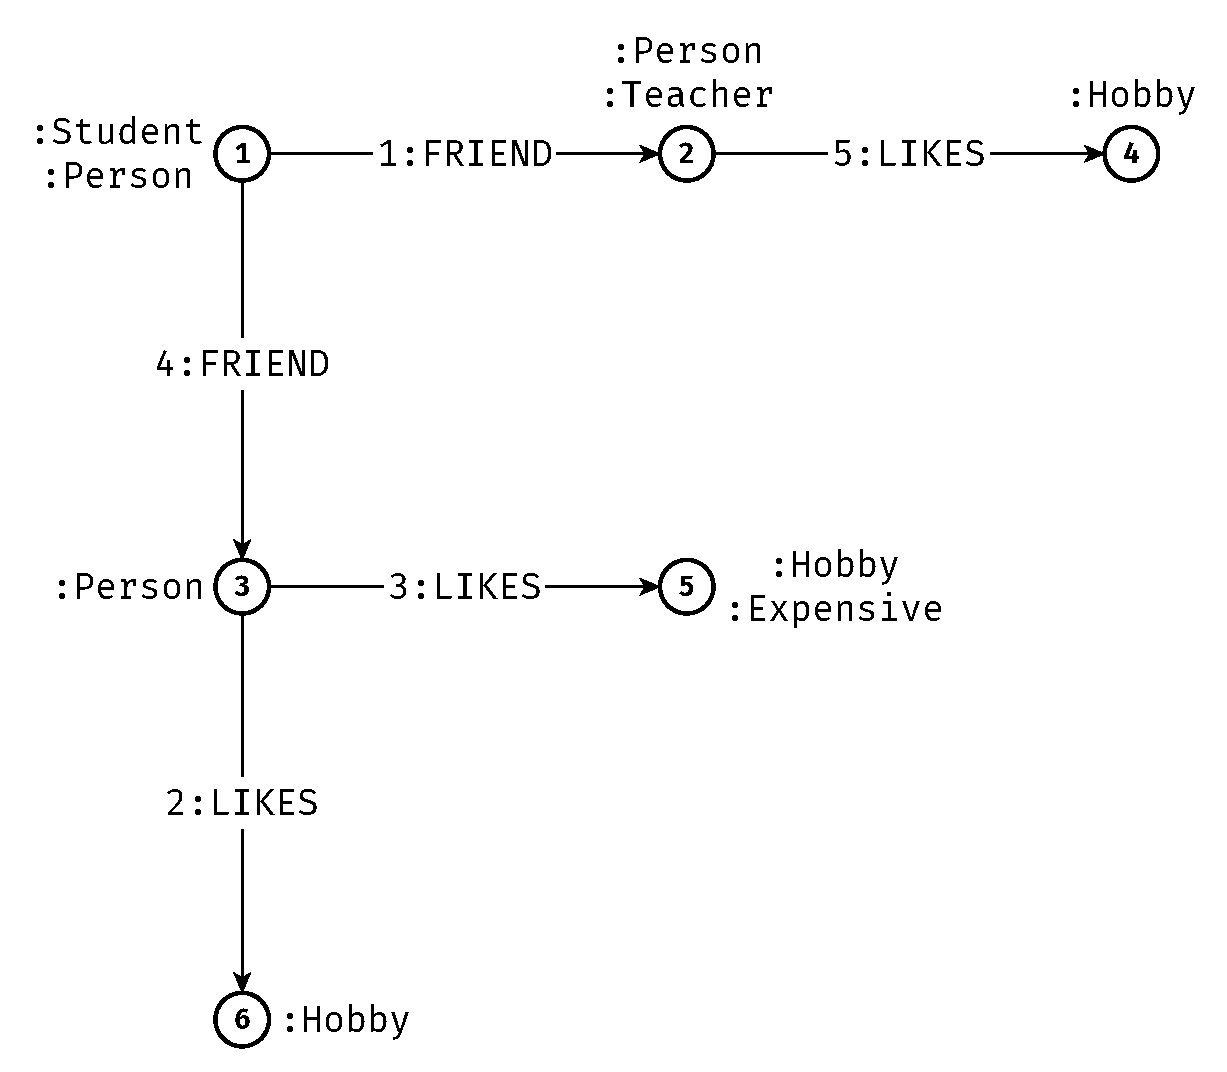
\includegraphics[width=0.7\textwidth]{figures/friend_likes_graph.pdf}
  \caption{A directed, labeled and typed multigraph.}
  \label{fig:dlt-graph}
\end{figure}

Figure \ref{fig:dlt-graph} shows an example database graph from a fictitious
social network. The function $\nlabel$ is encoded by writing all labels from
$\nlabel(v)$ next to the node $v$ in the graph, prefixed by a colon.
The function $\rtype$ is encoded by writing $\rtype(r)$ after each relationship
$r$ in the graph, separated by a colon.
In the example graph, nodes and relationships are identified by natural
numbers. It is required that nodes and relationships are disjoint. Therefore,
we write $x_n$ to refer to the node identified by the number $x$ and $x_r$ to
refer to the relationship identified by $x$.

\begin{remark}
In this thesis, we are only interested in the statistical information
derivable from node labels and relationship types.
We ignore that most graph databases additionally provide
a way of storing properties at nodes.

Node properties can be added to our graph model and to our query
algebra without any interference in the future.
\end{remark}

In a graph database system, queries return sets of subgraphs of the database $G$.
A subgraph can be defined in various ways. In its most general form, a subgraph
is a sequence of nodes of the database, together with a sequence of
relationships between these nodes.
Instead of natural numbers, we use a domain of query variables $\qvars$ to
enumerate the nodes and the relationships.

\begin{definition}[Subgraph]
Consider a domain of query variables $\qvars$. Let $X$ be a finite subset of
this domain.
A subgraph of the database $G$ is a function
$\mu ~:~ X \rightarrow V \union R$
such that
\[
  \forall r \in R ~~ \forall v_1 \in X ~~ (\mu(v_1) = r ~\Rightarrow~
    \exists v_2, v_3 \in X ~~ \lambda(r) = (\mu(v_2), \mu(v_3)))
\]

For $\mu(v) = x$ we say that $x$ is \emph{matched} by the variable $v$ in
the subgraph $\mu$.

We use the following set notation to write a subgraph
$\mu ~:~ \{v_1, \ldots, v_n\} \rightarrow V \union R$:
\[
  \mu = \{ v_1 \mapsto \mu(v_1), v_2 \mapsto \mu(v_2) \ldots, v_n \mapsto \mu(v_n) \}
\]


\end{definition}

In a \emph{query result} we want to collect all subgraphs having a
particular \emph{pattern}.
This pattern is defined as another graph, whose nodes and relationships consist
of query variables. The subgraphs having this pattern are all subgraphs that
are a graph homomorphism from the pattern graph to the database graph.
Our notion of graph homomorphism includes constraints on labels,
relationship types and on relationship uniqueness.

\begin{definition}[Subgraph pattern]
Like the database graph, a subgraph pattern is also a directed, labeled
and typed graph
$\rho = (V_\rho, R_\rho, \lambda_\rho, \nlabel_\rho, \rtype_\rho, \rpairs_\rho)$.

However, $\rtype_\rho$ does not map to one single relationship type,
but to a non-empty set of allowed relationship types:
\[
  \rtype_\rho ~:~ R_\rho \rightarrow \powSet{\rtypes} \setminus \emptyset
\]

Moreover, compared to the database graph, a subgraph pattern has one additional component:
\[
  \rpairs_\rho \subseteq \{ \{r, s\} \mid r,s \in R_\rho \land r \not = s \}
\]
This component will allow us to add uniqueness constraints on pairs of
relationship variables (see Definition \ref{def:query-result}).

Also, both nodes and relationships of a subgraph pattern are finite,
disjoint subsets of a domain of variables $\qvars$:
\begin{enumerate}
  \item $V_\rho \subseteq \qvars$
  \item $R_\rho \subseteq \qvars$
  \item $V_\rho \isect R_\rho = \emptyset$
\end{enumerate}
\end{definition}

The memory requirements of a subgraph pattern are shown in Table
\ref{table:subgraph-pattern-mem-reqs}.

\begin{table}
\centering
\begin{tabular}{ll}
\toprule
Component       & Space complexity                                                    \\ \midrule
$V_\rho$        & $O(\card{V_\rho})$                                                  \\[3pt]
$R_\rho$        & $O(\card{R_\rho})$                                                  \\[3pt]
$\lambda_\rho$  & $O(\card{R_\rho})$                                                  \\[3pt]
$\nlabel_\rho$  & $O(\card{V_\rho} \cdot \card{\nlabels})$                            \\[3pt]
$\rtype_\rho$   & $O(\card{R_\rho})$                                                  \\[3pt]
$\rpairs_\rho$  & $O(\binom{\card{R_\rho}}{2})$                                       \\[3pt]
\textbf{Total:} & $O(\binom{\card{R_\rho}}{2} + \card{V_\rho} \cdot \card{\nlabels})$ \\
\bottomrule
\end{tabular}
\caption{Space complexity of a subgraph pattern.}
\label{table:subgraph-pattern-mem-reqs}
\end{table}

The different components of a subgraph pattern can be best explained by
defining the corresponding query result.

\begin{definition}[Query result]
\label{def:query-result}
The query result $\result(\rho)$ of a subgraph pattern
$\rho = (V_\rho, R_\rho, \lambda_\rho, \nlabel_\rho, \rtype_\rho)$ is defined
as the set of all subgraphs
$\mu ~:~ V_\rho \union R_\rho \rightarrow V \union R$ that fulfil the
following constraints. For all $r,s \in  R_\rho$ and $v, w \in V_\rho$:
\begin{enumerate}[(1)]
  \item Node variables are only mapped to nodes and relationship variables only to relationships:
  
    $\mu(r) \in R$ and $\mu(v) \in V$
  \item Relationships between variables map to relationships in the database:
  
    $\lambda_\rho(r) = (v, w) \Rightarrow \lambda(\mu(r)) = (\mu(v), \mu(w))$
    
  \item The mapped nodes have at least the labels of the variables:
  
    $\nlabel_\rho(v) \subseteq \nlabel(\mu(v))$
    
  \item The mapped relationships are in the set of allowed types for the corresponding variable:
  
    $\rtype(\mu(r)) \in \rtype_\rho(r)$
    
  \item If two relationship variables are marked as disjoint, they map to
    different relationships:
    
    $\{r,s\} \in \rpairs_\rho \Rightarrow \mu(r) \not = \mu(s)$
\end{enumerate}
\end{definition}

\begin{figure}
  \centering
  
\includegraphics[width=0.7\textwidth]{figures/example-queries/person_p_friend_x_likes_z.pdf}
  \caption{A subgraph pattern and the corresponding query result in the
    database from Figure \ref{fig:dlt-graph}.}
  \label{fig:subgraph-pattern-1}
\end{figure}

Consider the subgraph pattern shown in red in Figure
\ref{fig:subgraph-pattern-1}.
Node and relationship variables are simply drawn from the alphabet.
Each relationship variable is assigned a set of allowed relationship types.
In the given example, these sets happen to consist of only one type.
Semantically, the example subgraph pattern produces all persons having a
friend who likes something. The subgraphs forming the corresponding query
result are shown in black. In set notation, the query result is given as:
\begin{align*}
  \{
    &\{ p \mapsto 1_n, f \mapsto 1_r, x \mapsto 2_n, l \mapsto 5_r, z \mapsto 4_n \} \\
    &\{ p \mapsto 1_n, f \mapsto 4_r, x \mapsto 3_n, l \mapsto 3_r, z \mapsto 5_n \} \\
    &\{ p \mapsto 1_n, f \mapsto 4_r, x \mapsto 3_n, l \mapsto 2_r, z \mapsto 6_n \}
  \}
\end{align*}

Let $\Omega$ be a query result and $\mu \in \Omega$. It is clear that
\[
  V_\rho = \{ v \mid \mu(v) \in V \}
    ~~~~
  R_\rho = \{ r \mid \mu(r) \in R \}
\]
for each subgraph pattern $\rho$ with $\result(\rho) = \Omega$.
This means that all subgraph patterns producing a query result do agree on
the set of node variables and relationship variables.

Therefore we can write these sets of node variables and relationship variables
as functions of $\Omega$:
\[
  \nvars(\Omega) := \{ v \mid \mu(v) \in V \land \mu \in \Omega \}
    ~~~~
  \rvars(\Omega) := \{ r \mid \mu(r) \in R \land \mu \in \Omega \}
\]

For convenience we also define
\[
  \vars(\Omega) := \nvars(\Omega) \union \rvars(\Omega)
\]

\section{The Algebra}
\label{sec:query-algebra}

Now that we have a notion of queries on a graph database (subgraph patterns)
and have defined the corresponding result sets, we are able to introduce a
query algebra.
The query algebra is defined on the space of all query results
\[
  \resultspace := \{ \result(\rho) \mid \rho \text{ is a subgraph pattern} \}
\]

All functions taking a finite number of query results as inputs and producing
another query result as output are possible operators of the algebra:
\[
 \operators := \{ o ~:~ \resultspace^k \rightarrow \resultspace \mid k \in \natnums_0 \}
\]

We will now define a set of operators and show their completeness, i.e., that every
query result can be produced by chaining these operators.

\section{Operators}
\label{sec:operators}

The \op{GetNodes} and \op{Expand} operators were first introduced by
Hölsch et al.\cite{holsch_algebra_2016}.

\begin{definition}[\op{GetNodes} operator]
\label{def:get-nodes}
The \op{GetNodes} operator $\getnodes{v}$ has no inputs and produces the set of
all single node subgraphs of the database $G$.

\begin{align*}
  \getnodes{v} &:= \{ \{ v \mapsto v' \} \mid v' \in V \}
\end{align*}

The subgraph pattern producing $\getnodes{v}$ is trivial:
\[
  \getnodes{v} = \result(
                   \{ v \},
                   \emptyset,
                   \emptyset \rightarrow \{v\}^2,
                   \{ v \mapsto \emptyset \},
                   \emptyset \rightarrow \powSet{\rtypes} \setminus \emptyset,
                   \emptyset)
\]

Therefore $\op{GetNodes}$ is a well-defined operator.
\end{definition}


\begin{definition}[\op{NodeJoin} operator]
\label{def:node-join}
The \op{NodeJoin} operator $\join$ takes two input query results with disjoint relationship variables
and merges them at the overlapping node variables.

Let $\mu_1 \in \Omega_1, \mu_2 \in \Omega_2$, $\rvars(\Omega_1) \isect \rvars(\Omega_2) = \emptyset$.
Merging the subgraphs $\mu_1$ and $\mu_2$ requires that their node matchings
are \emph{compatible} (denoted with $\mu_1 \sim \mu_2$):
\[
  \mu_1 \sim \mu_2 ~~\Leftrightarrow~~ \forall x \in \nvars(\Omega_1) \cap \nvars(\Omega_2): \mu_1(x)=\mu_2(x)
\]
We define the union of these subgraphs as
\[
  (\mu_1 \union \mu_2)(x) := \begin{cases}
                               \mu_1(x), \text{ if } x \in \vars(\mu_1), \\
                               \mu_2(x), \text{ otherwise }
                             \end{cases}
\]

Then we define the node join for all query results $\Omega_1, \Omega_2$
with $\rvars(\Omega_1) \isect \rvars(\Omega_2) = \emptyset$ as:
\begin{align*}
  \Omega_1 \join \Omega_2 &:= \{ \mu_1 \union \mu_2 \mid \mu_1 \in \Omega_1 \land \mu_2 \in \Omega_2 \land \mu_1 \sim \mu_2 \}
\end{align*}

\begin{proofof}{\op{NodeJoin} is a well-defined operator.}
\label{proof:node-join-well-defined}

Let $\Omega_1$ and $\Omega_2$ be query results and
$\rho_1 = (V_{\rho_1}, R_{\rho_1}, \lambda_{\rho_1}, \nlabel_{\rho_1}, \rtype_{\rho_1}, \rpairs_{\rho_1})$, 
$\rho_2 = (V_{\rho_2}, R_{\rho_2}, \lambda_{\rho_2}, \nlabel_{\rho_2}, \rtype_{\rho_2}, \rpairs_{\rho_2})$
be the corresponding subgraph patterns, i.e.
$\Omega_1 = \result(\rho_1)$ and $\Omega_2 = \result(\rho_2)$.

The precondition $\rvars(\Omega_1) \isect \rvars(\Omega_2) = \emptyset$ is
equivalent to $R_{\rho_1} \isect R_{\rho_2} = \emptyset$.

Let then $\rho = (V_\rho, R_\rho, \lambda_\rho, \nlabel_\rho, \rtype_\rho, \rpairs_\rho)$
with
\begin{itemize}[label={}]
  \item $V_\rho := V_{\rho_1} \union V_{\rho_2}$
  \item $R_\rho := R_{\rho_1} \union R_{\rho_2}$
  \item $\lambda_\rho ~:~ R_\rho \rightarrow {V_\rho}^2$ with
    $\lambda_\rho(r) := \begin{cases}
                          \lambda_{\rho_1}(r), \text{ if } r \in R_{\rho_1} \\
                          \lambda_{\rho_2}(r), \text{ if } r \in R_{\rho_2}
                        \end{cases}$
  \item $\nlabel_\rho(v) := L_1 \union L_2$ with
    $L_i := \begin{cases}
              \nlabel_{\rho_i}(v), \text{ if } v \in V_{\rho_i} \\
              \emptyset, \text{ otherwise }
            \end{cases}$ for $i \in \{1,2\}$
  \item $\rtype_\rho(r) := \begin{cases}
                             \rtype_{\rho_1}(r), \text{ if } r \in R_{\rho_1} \\
                             \rtype_{\rho_2}(r), \text{ if } r \in R_{\rho_2}
                           \end{cases}$
  \item $\rpairs_\rho := \rpairs_{\rho_1} \union \rpairs_{\rho_2}$
\end{itemize}

We do now have to show that every subgraph in $\Omega_1 \join \Omega_2$ is also
in $\result(\rho)$ and vice versa.

\begin{itemize}
  \item[$(\subseteq)$]
    Take $\mu \in \Omega_1 \join \Omega_2$. Then $\mu = \mu_1 \union \mu_2$ for
    some $\mu_1 \in \Omega_1$, $\mu_2 \in \Omega_2, \Omega_1 \sim \Omega_2$.
    
    We show that each constraint of Definition \ref{def:query-result} is fulfilled:
    \begin{enumerate}[(1)]
      \item % (1) Relationship variables are mapped to relationships and node variables to nodes
        Take $v \in V_\rho$ arbitrary. If $v \in V_{\rho_1}$ then $\mu(v) = \mu_1(v)$ and
        because $\mu_1 \in \Omega_1$ and $\Omega_1$ is a query result it holds that $\mu_1(v) \in V$.
        Analogously for $v \in V_{\rho_1}$.
        
        Take $r \in R_\rho$ arbitrary. If $r \in R_{\rho_1}$ then $\mu(r) = \mu_1(r)$ and
        because $\mu_1 \in \Omega_1$ and $\Omega_1$ is a query result it holds that $\mu_1(r) \in R$.
        Analogously for $r \in R_{\rho_2}$.
        
      \item % (2) Relationships between variables map to relationships in the database
        Assume $\lambda_\rho(r) = (v, w)$ for some $r \in R_{\rho_1}$ and $v,w \in V_\rho$.
        
        Then $\lambda_\rho(r) = \lambda_{\rho_1}(r) = (v, w)$. Because $\mu_1 \in \result(\rho_1)$
        it follows by constraint (2) that $\lambda(\mu_1(r)) = (\mu_1(v), \mu_1(w))$.
        
        Because $\Omega_1$ and $\Omega_2$ are compatible it holds that $\mu_1(x) = \mu(x)$ for all
        $x \in V_{\rho_1} \union R_{\rho_1}$. Therefore $\lambda(\mu(r)) = (\mu(v), \mu(w))$.
        
        Analogously for $r \in R_{\rho_2}$.
      
      \item % (3) The mapped nodes have at least the labels of the variables
        Take $v \in V_\rho$ arbitrary.
        
        If $v \in V_{\rho_1} \setminus V_{\rho_2}$
        then $\nlabel_\rho(v) = \nlabel_{\rho_1}(v) \subseteq \nlabel(\mu_1(v)) = \nlabel(\mu(v))$.
        
        Analogously for $v \in V_{\rho_2} \setminus V_{\rho_1}$.
        
        If $v \in V_{\rho_2} \isect V_{\rho_1}$
        then $\nlabel_\rho(v) = \nlabel_{\rho_1}(v) \union \nlabel_{\rho_2}(v)
          \subseteq \nlabel(\mu_1(v)) \union \nlabel(\mu_2(v)) = \nlabel(\mu(v))$.
      
      \item % (4) The mapped relationships are in the set of allowed types
        Take $r \in R_\rho$ arbitrary.
        
        If $r \in R_{\rho_1}$ then $\rtype_\rho(r) = \rtype_{\rho_1}(r) \ni \rtype(\mu_1(r)) = \rtype(\mu(r))$.
        
        Analogously for $r \in R_{\rho_2}$.
      
      \item % (5) Relationships are unique in each partition.
        Take $\{r,s\} \rpairs$ arbitrary.
        
        If $\{r,s\} \in \rpairs_{\rho_1}$, then
        $\mu(r) = \mu_1(r) \not = \mu_1(s) = \mu(s)$ because
        $\mu_1 \in \result(\rho_1)$.
        
        Analogously for $\{r,s\} \in \rpairs_{\rho_2}$.
    \end{enumerate}
  
  Therefore $\mu \in \result(\rho)$.
  
  \item[$(\supseteq)$]
    Take $\mu \in \result(\rho)$.
    
    Let $\mu_1 ~:~ V_{\rho_1} \union R_{\rho_1} \rightarrow V \union R$ with $\mu_1(x) := \mu(x)$
    and $\mu_2 ~:~ V_{\rho_2} \union R_{\rho_2} \rightarrow V \union R$ with $\mu_2(x) := \mu(x)$.
    
    Then $\mu_1 \in \result(\rho_1) = \Omega_1$ and $\mu_2 \in \result(\rho_2) = \Omega_2$.
    
    Also $\mu_1 \sim \mu_2$.
    
    Therefore $\mu \in \Omega_1 \join \Omega_2$.
\end{itemize}

We have shown that, for any input results $\Omega_1 = \result(\rho_1)$,
$\Omega_2 = \result(\rho_2)$, there is a subgraph pattern $\rho$ with
$\result(\rho) = \Omega_1 \join \Omega_2$.

Therefore \op{NodeJoin} is a well-defined query operator mapping from
$\resultspace^2$ to $\resultspace$.
\end{proofof}
\end{definition}

\begin{example}
  \newcommand{\pfriendofx}{\vcenter{\hbox{
\includegraphics[height=2.6ex]{figures/subgraph-patterns/person_p_friend_x.pdf}}}}
  \newcommand{\xlikesz}{\vcenter{\hbox{
\includegraphics[height=2.6ex]{figures/subgraph-patterns/x_likes_z.pdf}}}}
  \newcommand{\pfriendofxlikesz}{\vcenter{\hbox{
\includegraphics[height=2.6ex]{figures/subgraph-patterns/person_p_friend_x_likes_z.pdf}}}}
  
  It holds that
  \begin{align*}
    &\result(\pfriendofx) \join \result(\xlikesz) \\
    &~~ = \result(\pfriendofxlikesz)
  \end{align*}
\end{example}



\begin{definition}[\op{Traverse} operator]
\label{def:traverse}

The \op{Traverse} operator $\traversevar{v}{r:T}{\alpha}{w}(\Omega)$ takes a query
result $\Omega$ as input and expands it by adding new relationships between nodes.
The precondition is that $v,w \in \nvars(\Omega)$.
The direction of the relationships is specified by
$\alpha \in \{\leftarrow, \rightarrow\}$
and the allowed relationship types by
$T \subseteq \rtypes$.

For $\lambda(s) = (p, q)$ we set $\lambda_\rightarrow(s) = (p, q)$ and
$\lambda_\leftarrow(s) = (q, p)$.

Then we define
\begin{align*}
  \traversevar{v}{r:T}{\alpha}{w}(\Omega) := \{ &\mu \union \{ r \mapsto r' \} \mid
    \mu \in \Omega \land \lambda_\alpha(r') = (\mu(v), \mu(w)) \land t(r') \in T \}
\end{align*}

\begin{proofof}{\op{Traverse} is a well-defined operator.}
\label{proof:traverse-well-defined}

Let $\Omega$ be a query result and
$\rho' = (V_{\rho'}, R_{\rho'}, \lambda_{\rho'}, \nlabel_{\rho'}, \rtype_{\rho'}, \rpairs_{\rho'})$
the corresponding subgraph pattern.

Let then $\rho = (V_\rho, R_\rho, \lambda_\rho, \nlabel_\rho, \rtype_\rho, \rpairs_\rho)$
with
\begin{itemize}[label={}]
  \item $V_\rho := V_{\rho'}$
  \item $R_\rho := R_{\rho'} \union \{ r \}$
  \item $\lambda_\rho(x) := \begin{cases}
                              (v, w) \text{ if } x = r ~\land~ \alpha = \rightarrow \\
                              (w, v) \text{ if } x = r ~\land~ \alpha = \leftarrow \\
                              \lambda_{\rho'}(x), \text{ otherwise}
                            \end{cases}$
  \item $\nlabel_\rho := \nlabel_{\rho'}$
  \item $\rtype_\rho(x) := \begin{cases}
                              T, \text{ if } x = r \\
                              \rtype_{\rho'}(x), \text{ otherwise}
                           \end{cases}$
  \item $\rpairs_\rho := \rpairs_{\rho'}$
\end{itemize}

Again we have to show that every subgraph in
$\traversevar{v}{r:T}{\alpha}{w}(\Omega)$ is also in $\result(\rho)$ and vice
versa.

\begin{itemize}
  \item[$(\subseteq)$]
    Take $\mu \in \traversevar{v}{r:T}{\alpha}{w}(\Omega)$ arbitrary.
    Then $\mu = \mu' \union \{ r \mapsto r' \}$ for some $\mu' \in \Omega$,
    $r' \in R$, such that $\lambda_\alpha(r') = (\mu'(v), \mu'(w'))$.
    
    We show again that each constraint of Definition \ref{def:query-result} is
    fulfilled:
    \begin{enumerate}[(1)]
      \item % (1) Node variables are mapped to nodes and relationship variables
            % to relationships
        $\mu(r) = r' \in R$ by definition.
        For all $v \in V_\rho, s \in R_\rho \setminus \{r\}$:
        $\mu(v) = \mu'(v) \in V$ and $\mu(s) = \mu'(s) \in R$ because
        $\mu' \in \Omega$ and $\Omega$ is a query result.
      \item % (2) Relationships between variables map to relationships in the
            %     database
        If $\alpha = \rightarrow$
        then $\lambda_\rho(r) = (v, w)$
        and $\lambda(\mu(r)) = \lambda(r') = \lambda_\rightarrow(r')
                             = (v', w') = (\mu(v), \mu(w))$.
        
        If $\alpha = \leftarrow$
        then $\lambda_\rho(r) = (w, v)$
        and $\lambda(\mu(r)) = \lambda(r') = \lambda_\rightarrow(r')
                             = (w', v') = (\mu(w), \mu(v))$.
        
        For $x \in R_\rho, x \not = r$ it holds that if
        $\lambda_\rho(x) = \lambda_{\rho'}(x) = (p, q)$
        then $\lambda(\mu(x)) = \lambda(\mu'(x))
                              = (\mu'(p), \mu'(q)) = (\mu(p), \mu(q))$
        because $\mu' \in \Omega$ and $\Omega$ is a query result.
        
      \item % (3) The mapped nodes have at least the labels of the variables
        Take $v \in V_\rho$ arbitrary.
        $\nlabel_\rho(v) = \nlabel_{\rho'}(v) \subseteq \nlabel(\mu'(v))
                         = \nlabel(\mu(v))$.
      
      \item % (4) The mapped relationships are in the set of allowed types
        $\rtype_\rho(r) = T \ni t(r') = t(\mu(r))$ by definition.
        
        For $s \in R_\rho, s \not = r$ it holds that
        $\rtype_\rho(s) = \rtype_{\rho'}(s) \ni \rtype(\mu'(s)) = \rtype(\mu(s))$.
      
      \item % (5) Relationships are mapped different if they are marked different.
        Take $\{s,t\} \in \rpairs_\rho = \rpairs_{\rho'}$ arbitrary.
        Then $s,t \in R_{\rho'}$ and therefore $\mu(s) = \mu'(s)$ and
        $\mu(t) = \mu'(t)$.
        
        Because $\mu' \in \result(\rho')$ it follows that
        $\mu(s) = \mu'(s) \not = \mu'(t) = \mu(t)$.
    \end{enumerate}
    
    As a result, $\mu \in \result(\rho)$.

  \item[$(\supseteq)$]
    Take $\mu \in \Omega = \result(\rho)$ arbitrary. Let
    $\mu' ~:~ V_{\rho'} \union R_{\rho'} \rightarrow V \union R$ with
    $\mu'(x) := \mu(x)$.
    Then $\mu' \in \result(\rho') = \Omega$.
    
    If $\alpha = \rightarrow$
    then $\lambda_\rho(r) = (v, w)$
    and because of constraint (2)
    $\lambda_\alpha(\mu(r)) = \lambda(\mu(r)) = (\mu(v), \mu(w))$.
    
    Analogously for $\alpha = \leftarrow$.
    
    Finally, $\rtype(r') = \rtype(\mu(r)) \in \rtype_\rho(r) = T$.
    
    Therefore, $\mu \in \traversevar{v}{r:T}{\alpha}{w}(\Omega)$.
\end{itemize}

It follows that $\traversevar{v}{r:T}{\alpha}{w}(\Omega) = \result(\rho)$.
We conclude that \op{Traverse} is a well-defined operator.
\end{proofof}
\end{definition}



\begin{definition}[\op{Expand} operator]
\label{def:expand}

The \op{Expand} operator $\expandvar{v}{r:T}{\alpha}{w}(\Omega)$ takes a query
result $\Omega$ as input and expands it by adding new nodes using
relationships. The preconditions are that
$v \in \nvars(\Omega)$
and
$w \not \in \nvars(\Omega)$
The direction of the relationships is specified by
$\alpha \in \{\leftarrow, \rightarrow\}$
and the allowed relationship types by
$T \subseteq \rtypes$.

For $\lambda(r) = (v, w)$ we set $\lambda_\rightarrow(r) = (v, w)$ and
$\lambda_\leftarrow(r) = (w, v)$.

Then we define
\[
  \expandvar{v}{r:T}{\alpha}{w}(\Omega) := \{ \mu \union \{ r \mapsto r', w \mapsto w' \} \mid
                                              \mu \in \Omega \land \lambda_\alpha(r') = (\mu(v), \mu(w))
                                              \land \rtype(r') \in T \}
\]

\begin{proofof}{\op{Expand} is a well-defined operator.}
\label{proof:expand-well-defined}

By definition it holds that
\begin{align}
\begin{split}
  \expandvar{v}{r:T}{\alpha}{w}(\Omega) &= \{ \mu \union \{ r \mapsto r' \} \union \{ w \mapsto w' \} \mid
                                              \mu \in \Omega \land \lambda_\alpha(r') = (\mu(v), \mu(w))
                                              \land \rtype(r') \in T \} \\
                                        &= \{ \mu_1 \union \mu_2 \union \{ r \mapsto r' \} \mid
                                              \mu_1 \in \Omega \land \mu_2 \in \getnodes{w} \land \lambda_\alpha(r') = (\mu_1(v), \mu_2(w))
                                              \land \rtype(r') \in T \} \\
                                        &= \{ \mu \union \{ r \mapsto r' \} \mid
                                              \mu \in \Omega \join \getnodes{w} \land \lambda_\alpha(r') = (\mu(v), \mu(w))
                                              \land \rtype(r') \in T \} \\
                                        &= \traversevar{v}{r:T}{\alpha}{w}(\Omega \join \getnodes{w}) \label{eq:expand}
\end{split}
\end{align}

Because the operators \op{GetNodes}, \op{Join} and \op{Traverse} are well-defined, the \op{Expand} operator
is also well-defined.
\end{proofof}

\begin{remark}
Because the \op{Expand} operator can be defined in terms of \op{GetNodes},
\op{Join} and \op{Traverse}, it is not needed from a logical perspective.

However, some graph databases (e.g. Neo4j) provide special physical operators
implementing the \op{Expand} operator in an efficient manner. Thus there is
an interest in having this operator available as a shorthand for the combination
of canonical operators shown in Equation \ref{eq:expand}.
\end{remark}
\end{definition}

\begin{example}
  \newcommand{\teachert}{\vcenter{\hbox{
\includegraphics[height=2.6ex]{figures/subgraph-patterns/teacher_t.pdf}}}}
  \newcommand{\pfriendoft}{\vcenter{\hbox{
\includegraphics[height=2.6ex]{figures/subgraph-patterns/p_friend_teacher_t.pdf}}}}
  
  It holds that
  \[
    \expandin{t}{f:\{\text{FRIEND}\}}{p}(\result(\teachert)) = \result(\pfriendoft)
  \]
\end{example}


\begin{definition}[\op{LabelSelection} operator]
\label{def:label-selection}

The \op{LabelSelection} operator $\selection{v:l}(\Omega)$ takes a query
result $\Omega$ as input and returns only those subgraphs where the node
matched by $v$ has the label $l$.

It is defined as
\begin{align*}
  \selection{v:l}(\Omega) := \{ \mu \in \Omega \mid l \in \nlabel(\mu(v)) \}
\end{align*}

\begin{proofof}{\op{LabelSelection} is a well-defined operator.}
\label{proof:label-selection-well-defined}

Let $\Omega$ be a query result and
$\rho' = (V_{\rho'}, R_{\rho'}, \lambda_{\rho'}, \nlabel_{\rho'}, \rtype_{\rho'}, \rpairs_{\rho'})$
the corresponding subgraph pattern.

Let then $\rho = (V_\rho, R_\rho, \lambda_\rho, \nlabel_\rho, \rtype_\rho, \rpairs_\rho)$
with
\begin{itemize}[label={}]
  \item $V_\rho := V_{\rho'}$
  \item $R_\rho := R_{\rho'}$
  \item $\lambda_\rho := \lambda_{\rho'}$
  \item $\nlabel_\rho(x) := \begin{cases}
                              \nlabel_{\rho'} \union \{ l \}, \text{ if } x = v \\
                              \nlabel{\rho'}(x), \text{ otherwise}
                            \end{cases}$
  \item $\rtype_\rho := \rtype_{\rho'}$
  \item $\rpairs_\rho := \rpairs_{\rho'}$
\end{itemize}

Once more we have to show that every subgraph in
$\selection{v:l}(\Omega)$ is also in $\result(\rho)$ and vice
versa.

\begin{itemize}
  \item[$(\subseteq)$]
    Take $\mu \in \selection{v:l}(\Omega)$ arbitrary.
    Then $\mu \in \Omega$ with $l \in \nlabel(\mu(v))$.
    
    We show again that each constraint of Definition \ref{def:query-result} is
    fulfilled (but with less detail, to avoid repetition):
    \begin{enumerate}[(1)]
      \item % (1) Node variables are mapped to nodes and relationship variables
            % to relationships
        Fulfilled, because $\mu \in \Omega$ and $\Omega$ is a query result.
        
      \item % (2) Relationships between variables map to relationships in the
            %     database
        Fulfilled, because $\lambda_\rho = \lambda_{\rho'}$ and
        $\mu \in \result(\rho')$.
        
      \item % (3) The mapped nodes have at least the labels of the variables
        First of all, by definition $\{l\} \subseteq \nlabel(\mu(v))$.
        Also $\nlabel_{\rho'}(v) \subseteq \nlabel(\mu(v))$, because
        $\mu \in \Omega$ and $\Omega$ is a query result.
        Therefore, $\nlabel_\rho(v) = \{l\} \union \nlabel_{\rho'}(v)
                                    \subseteq \nlabel(\mu(v))$
      
      \item % (4) The mapped relationships are in the set of allowed types
        Fulfilled, because $\rtype_\rho = \rtype_{\rho'}$ and
        $\mu \in \result(\rho')$.
        
      \item % (5) Relationships are unique in each partition.
        Fulfilled, because and $\rpairs_\rho = \rpairs_{\rho'}$ and
        $\mu \in \result(\rho')$.
    \end{enumerate}
    
    As a result, $\mu \in \result(\rho)$.

  \item[$(\supseteq)$]
    Take $\mu \in \result(\rho)$ arbitrary.
    Then $\mu \in \result(\rho') = \Omega$, because the subgraph pattern $\rho$
    has a superset of the constraints of $\rho'$.
    
    Also $\nlabel_\rho(v) = \nlabel_{\rho'}(v) \union \{l\}
                          \subseteq \nlabel(\mu(v))$
    which implies that $l \in \nlabel(\mu(v))$.
    
    Therefore, $\mu \in \selection{v:l}(\Omega)$.
\end{itemize}

We have proven that $\selection{v:l}(\Omega) = \result(\rho)$ and conclude that
\op{LabelSelection} is a well-defined operator.
\end{proofof}
\end{definition}

\begin{definition}[\op{DistinctSelection} operator]
\label{def:distinct}

The \op{DistinctSelection} operator $\distinct{r}{s}(\Omega)$ takes a query
result $\Omega$ as input and returns only those subgraphs where the
relationships matched by the variables $r$ and $s$ are different.

It is defined as
\begin{align*}
  \distinct{r}{s}(\Omega) := \{ \mu \in \Omega \mid \mu(r) \not = \mu(s) \}
\end{align*}

\begin{proofof}{\op{DistinctSelection} is a well-defined operator.}
\label{proof:distinct-well-defined}

Let $\Omega$ be a query result and
$\rho' = (V_{\rho'}, R_{\rho'}, \lambda_{\rho'}, \nlabel_{\rho'}, \rtype_{\rho'}, \rpairs_{\rho'})$
the corresponding subgraph pattern.

Let then $\rho = (V_\rho, R_\rho, \lambda_\rho, \nlabel_\rho, \rtype_\rho, \rpairs_\rho)$
with
\begin{itemize}[label={}]
  \item $V_\rho := V_{\rho'}$
  \item $R_\rho := R_{\rho'}$
  \item $\lambda_\rho := \lambda_{\rho'}$
  \item $\nlabel_\rho := \nlabel_{\rho'}$
  \item $\rtype_\rho := \rtype_{\rho'}$
  \item $\rpairs_\rho := \rpairs_{\rho'} \union \{ \{ r,s \} \}$
\end{itemize}

Once more we have to show that every subgraph in
$\distinct{r}{s}(\Omega)$ is also in $\result(\rho)$ and vice
versa.

\begin{itemize}
  \item[$(\subseteq)$]
    Take $\mu \in \distinct{r}{s}(\Omega)$ arbitrary.
    Then $\mu \in \Omega$ with $\mu(r) \not = \mu(s)$.
    
    We show again that each constraint of Definition \ref{def:query-result} is
    fulfilled:
    \begin{enumerate}[(1)]
      \item % (1) Node variables are mapped to nodes and relationship variables
            % to relationships
        Fulfilled, because $\mu \in \Omega$ and $\Omega$ is a query result.
        
      \item % (2) Relationships between variables map to relationships in the
            %     database
        Fulfilled, because $\lambda_\rho = \lambda_{\rho'}$ and
        $\mu \in \result(\rho')$.
        
      \item % (3) The mapped nodes have at least the labels of the variables
        Fulfilled, because $\nlabel_\rho = \nlabel_{\rho'}$ and
        $\mu \in \result(\rho')$.
      
      \item % (4) The mapped relationships are in the set of allowed types
        Fulfilled, because $\rtype_\rho = \rtype_{\rho'}$ and
        $\mu \in \result(\rho')$.
        
      \item % (5) Relationship variables are mapped to different relationships
            %     if they are marked different
        By definition it holds that $\{r,s\} \in \rpairs_\rho$ and
        $\mu(r) \not = \mu(s)$.
        
        Take now $\{t,u\} \in \rpairs_\rho$ with $\{t,u\} \not = \{r,s\}$.
        Then $\{t,u\} \in \rpairs_{\rho'}$ and because $\mu \in \result(\rho')$
        it follows that $\mu(t) \not = \mu(u)$.
    \end{enumerate}
    
    As a result, $\mu \in \result(\rho)$.

  \item[$(\supseteq)$]
    Take $\mu \in \result(\rho)$ arbitrary.
    Then $\mu \in \result(\rho') = \Omega$, because the subgraph pattern $\rho$
    has a superset of the constraints of $\rho'$.
    Because $\{r,s\} \in \rpairs_\rho$, we have $\mu(r) \not = \mu(s)$.
    
    Therefore, $\mu \in \distinct{r}{s}(\Omega)$.
\end{itemize}

We have proven that $\distinct{r}{s}(\Omega) = \result(\rho)$ and conclude that
\op{DistinctSelection} is a well-defined operator.
\end{proofof}
\end{definition}

\section{Completeness}
\label{sec:completeness}

A set of operators is \emph{complete}, iff it is possible to produce the whole
result space of the corresponding algebra by chaining these operators.

We are interested in the set
\[
  \operators_c := \{ \getnodes{v}, \join, \traversevar{v}{r:T}{\alpha}{w},
                     \selection{v:l}, \distinct{r}{s} \} \subset \operators
\]

\begin{proofof}{$\operators_c$ is a complete set of operators w.r.t.
                $\resultspace$.}
  Let $\rho = (V_\rho, R_\rho, \lambda_\rho, \nlabel_\rho, \rtype_\rho, \rpairs_\rho)$ be a
  subgraph pattern. We have to show that there is a combination of query
  operators from $\operators_c$ producing $\result(\rho)$.
  
  First of all, because $V_\rho, R_\rho$ are finite, we can enumerate them in
  a sequence:
  \[
    V_\rho = \{ v_1, v_2, \ldots, v_\card{V_\rho} \}, ~~ R_\rho = \{ r_1, r_2, \ldots, r_\card{R_\rho} \}
  \]
  
  The same holds for all labels of a node variable $v_i \in V_\rho$
  \[
    \nlabel_\rho(v_i) = \{ l_{i,1}, l_{i,2}, \ldots, l_{i,\card{\nlabel_\rho(v_i)}} \}
  \]
  and for all pairs of relationships in $\rpairs_\rho$
  \[
    \rpairs_\rho = \{ \{r_{1,1}, r_{1,2}\}, \ldots, \{r_{\card{\rpairs_\rho},1}, r_{\card{\rpairs_\rho},2}\} \}
  \]
  
  We can now reuse some work done in the previous proofs, where we showed that
  the query operators are well-defined.
  For each operator we defined an output subgraph pattern in terms of the
  input subgraph patterns. The idea for the completeness proof is the
  following:
  We build a chain of query operators which we suppose to equal
  $\result(\rho)$. Then we use the mentioned pattern definitions to find a
  pattern $\rho'$ that produces the same query result as this chain.
  We will see that $\rho' = \rho$ and therefore
  $\result(\rho') = \result(\rho)$.
  
  Let us start to build the chain of operators.
  
  \begin{enumerate}
    \item % 1. Matching single nodes.
      We begin with the following query result: 
      \begin{align*}
        J_1 &:= \getnodes{v_1} \\
        J_i &:= \getnodes{v_i} \join J_{i-1}
          ~~\text{ for } i \in \{ 2, \ldots, \card{V_\rho} \}
      \end{align*}
      
      In Definition \ref{def:get-nodes} we found that,
      $J_1 = \getnodes{v_1}$ can be produced by a pattern that has only one node variable,
      no relationships and no type or label constraints.
      Using Definition \ref{def:node-join} we observe that, given a pattern $\rho_{i-1}$
      producing $J_{i-1}$, a pattern $\rho_i$ producing $J_i$ can be obtained by simply
      adding the variable $v_i$ to the set of nodes of $\rho_{i-1}$.
      All other components of $\rho_i$ equal those of $\rho_{i-1}$.
      
      Consequently, the following pattern $\rho_J$ having all node variables
      $V_\rho$ but no relationships, no type constraints and no label
      constraints will produce $J_\card{V_\rho}$:
      
      $\rho_J = (V_\rho, \emptyset, \emptyset \rightarrow {V_\rho}^2,
       V_\rho \rightarrow \emptyset,
       \emptyset \mapsto \powSet{\rtypes} \setminus \emptyset,
       \emptyset)$.
      
   \item % 2. Matching relationships:
      In the next step, we match relationships between the nodes in
      $J_\card{V_\rho}$.
      
      For a tuple $t = (t_1, t_2, \ldots, t_n)$ we denote the projection on the
      $i$'th component with $\pi_i(t) := t_i$.
      
      We construct a sequence of \op{Traverse} operators matching all
      relationships that exist in $\rho$:
      \begin{align*}
        R_0 &:= J_\card{V_\rho} \\
        R_i &:= \traverseout{\pi_1(\lambda_\rho(r_i))}{r_i:\rtype_\rho(r_i)}{
          \pi_2(\lambda_\rho(r_i))}(R_{i-1})
      \end{align*}
      
      Incrementing the parameter from $i-1$ to $i$ means to append a
      \op{Traverse} operator for relationship $r_i$ to $R_{i-1}$.
      According to the proof that \op{Traverse} is well-defined
      (cf. Definition \ref{def:traverse}), this is equivalent to adding the relationship $r_i$
      to the corresponding subgraph pattern, together with the type constraint.
      
      It is easy to see that, $R_\card{R_\rho} = \result(\rho_R)$ with
      $\rho_R = (V_\rho, R_\rho, \lambda_\rho,
       V_\rho \rightarrow \{ \emptyset \},
       \rtype_\rho,
       \rpairs_\rho)$.
      This pattern already equals $\rho$ in all components except the label
      function and the set of distinct relationship pairs.
      
    \item % 3. Selecting by labels
      In the second last step, we shrink the set of subgraphs by adding label constraints.
      
      We define
      \begin{align*}
        L_{0,0} &:= R_\card{R_\rho} \\
        L_{i,0} &:= L_{i-1, \card{\nlabel_\rho(v_i)}}
          ~~\text{ for } i \in \{ 1, \ldots, \card{V_\rho} \} \\
        L_{i,j} &:= \selection{v_i:l_{i,j}}(L_{i,j-1})
          ~~\text{ for } i \in \{ 1, \ldots, \card{V_\rho} \},
                         j \in \{ 1, \ldots, \card{\nlabel(v_i)} \}
      \end{align*}
      
      We are interested in
      $L := L_{\card{V_\rho}, \card{\nlabel_\rho(v_\card{V_\rho})}}$.
      As in the previous two steps, we iteratively construct a subgraph pattern
      which produces the same result, using the recursive definition from the
      proof that the \op{LabelSelection} operator is well-defined
      (cf. Definition \ref{def:label-selection}).
      
      Going from $L_{i,j}$ to $L_{i,j-1}$ means to append a \op{LabelSelection}
      for label $l_{i,j}$ on the node variable $v_i$.
      According to the proof that \op{LabelSelection} is well-defined
      (cf. Definition \ref{def:label-selection}), this is equivalent to adding a new label
      to $\nlabel(v_i)$ in the corresponding subgraph pattern.
      All other components of the pattern do not change.
      
      We see that $L$
      contains exactly one \op{LabelSelection} for each label constraint stored
      in $\nlabel_\rho$.
      Therefore, going from the previous pattern $\rho_R$ to a pattern $\rho_L$
      with $\result(\rho_L) = L$,
      means adding all of the label constraints from $\nlabel_\rho$ to
      $\rho_R$. Because there are no label constraints in $\rho_R$, the label
      function in $\rho_L$ simply equals $\nlabel_\rho$.
      
      Thus the generated pattern is
      \[
         \rho_L = (V_\rho, R_\rho, \lambda_\rho, \nlabel_\rho, \rtype_\rho, \emptyset)
      \]
      
    \item % 4. Selecting distinct relationships
      In the final step, we shrink the set of subgraphs by introducing
      constraints ensuring relationship uniqueness.
      
      We define
      \begin{align*}
        U_0 &:= L \\
        U_i &:= \distinct{r_{i,1}}{r_{i,2}}(U_{i-1})
          ~~\text{ for } i \in \{ 1, \ldots, \card{\rpairs_\rho} \}
      \end{align*}
      
      We are interested in $U := U_\card{\rpairs_\rho}$.
      We proceed as in the previous steps.
      
      Going from $U_i$ to $U_{i-1}$ means to append a \op{DistinctSelection} operator
      for the relationships $r_{i,1}, r_{i,2}$.
      According to the proof that \op{DistinctSelection} is well-defined
      (cf. Definition \ref{def:distinct}), this is equivalent to adding the pair
      $\{r_{i,1}, r_{i,2}\}$ to the set of distinct relationship pairs in the
      corresponding subgraph pattern.
      All other components of the pattern do not change.
      
      We see that $U$ contains exactly one \op{DistinctSelection} operator for each
      pair of relationship variables stored in $\rpairs_\rho$.
      Therefore, going from the previous pattern $\rho_L$ to $\rho_U$
      with $\result(\rho_U) = U$, means adding all of the pairs from
      $\rpairs_\rho$ to $\rho_L$.
      Because the set of distinct relationship pairs of $\rho_L$ is empty, the
      set of distinct relationship pairs of $\rho_U$ simply equals
      $\rpairs_\rho$.
      
      Thus the generated pattern is
      \[
         \rho_U = (V_\rho, R_\rho, \lambda_\rho, \nlabel_\rho, \rtype_\rho, \rpairs_\rho) = \rho
      \]
      
      It follows that
      \[
        U = \result(\rho_U) = \result(\rho) ~\text{.}
      \]
  \end{enumerate}
\end{proofof}

% \section{Graph query languages}
%
% \begin{definition}[Graph query language]
% Take  a finite set of graph query operators $O_L \subset \operators$.
%
% The corresponding query language 
% \end{definition}


\chapter{Assumptions About the Distribution of Labels}
\chaptermark{Label Assumptions}
\label{chap:label-assumptions}

\begin{aboutchapter}
In this chapter, we introduce three possible assumptions about the distribution
of node labels and show that none of them is likely to be valid for the
whole database.
To address this problem, we propose two data structures to decide which
assumption to use for a particular set of labels.
\end{aboutchapter}

% \section{Using node labels and relationship types for the estimation of logical
%          result properties}
% \label{sec:node-labels-for-estimation}
%
% As pointed out, node labels are a way for the user to assign a meaning to
% particular groups of nodes. Two nodes having the same label are part of the
% same semantic population defined by the user. It can therefore be assumed that,
% nodes having a particular label tend to share some properties.
%
% With this observation in mind, it seems sensible to base the estimation of
% logical result properties on information corresponding to sets of nodes having
% particular labels.
%
% Additionally, as mentioned before, it can be assumed that the user tends to
% formulate queries which select exactly all nodes having one or several labels.
% Storing helpful information corresponding to these labels allows to estimate
% the logical result properties for such queries very precisely.
%
% Similar arguments can be made in favor of using information corresponding to
% particular relationship types. However, because relationships are defined as
% ordered pairs of nodes, they have to be understood as additional information on
% the nodes in the graph and not as an individual concept.
% It can therefore be argued that, information on relationship types is most
% valuable in conjunction with information on the nodes being connected 
% by the corresponding relationships, i.e. with information on the node labels of
% the connected nodes.
% This argument explains the wide-spread usage of triple statistics
% $(l_1, t, l_2)$ storing the number of relationships of type $t$ starting at
% nodes with label $l_1$ and ending at nodes with label $l_2$, for all labels
% $l_1, l_2$ and relationship types $t$.
%
% To summarize, we will use information corresponding to particular labels and
% relationship types in our estimations.

\section{The Problem of Global Assumptions}
\sectionmark{Global Assumptions}

In the relational algebra, a result of tuples can be filtered according to a
predicate $p$ using the selection operator $\sigma_p$.
Estimating the result cardinality of the selection is equivalent to estimating
the probability of the predicate.

To estimate the probability of a predicate that references multiple attributes,
it is essential to know how the value combinations of these attributes are distributed.
A simple approach is to assume probabilistic independence of the attributes.
The probability of a combination of attribute values is then simply the product
of the individual value probabilities, which are stored in the system catalog.

However, the attribute value independence assumption is often violated in real
data sets (e.g. when there are functional dependencies).
Consequently, research has been done to find better ways of estimating the result
cardinality of multi-attribute selections \cite{poosala_selectivity_1997}.

In our graph algebra, nodes can be filtered using the \op{NodeLabelSelection}
operator.
Suppose the graph DBMS maintains a relation $R$ with schema
$<n, l_1, \ldots, l_i>$, where $n$ is a node and $l_1, \ldots, l_i$ are
Booleans assigning a set of labels to this node.
Estimating the result cardinality of several consecutive label
selections is then equivalent to estimating the result cardinality of a multi-
attribute selection on the $l_1, \ldots, l_i$ attributes of this table.
Consequently, label selections in a graph database can be viewed as a special
case of multi-attribute selections in a relational database.

Take for instance two labels called "Person" and "Student".
Semantically, every student is a person. Therefore
$\selection{v:\text{Student}}(\selection{v:\text{Person}}(\getnodes{v}))
  = \selection{v:\text{Student}}(\getnodes{v})$.
We say that "Student" is a sublabel of "Person" (see Definition
\ref{def:sublabel}).
Obviously, if the database knows about this sublabel relationship, it will make
a far better estimation of the result cardinality than if it assumes e.g.,
independence of students and persons.

\begin{remark}
Relationship types resemble node labels, because they
are also a way of assigning a group membership to a set of entities,
namely relationships.
However, every relationship is exactly of one type. As a result, there is no
uncertainty about the distribution of relationship types, they are disjoint
(unlike node labels).
\end{remark}

Nevertheless, the popular graph database Neo4j always assumes independence
of labels.
In this thesis, we want to demonstrate that cardinality estimates can be
significantly improved by incorporating more information about the node label
distribution. In particular, we consider the cases that labels are
\emph{disjoint} or
in a \emph{sublabel} relation.

\begin{definition}[Sublabels]
\label{def:sublabel}
A label $l'$ is a sublabel of $l$, iff
$\selection{v:l'}(\getnodes{v}) \subseteq \selection{v:l}(\getnodes{v})$.
Equivalently, we call $l$ a superlabel of $l'$.
We denote this relation by $l' \subseteq l$.
\end{definition}

Let us now formalize possible assumptions on the node label distribution.

Take a query result $\Omega$. $\Omega$ can be interpreted as a finite
probability space, such that each subgraph $\mu \in \Omega$ is an elementary
event with probability $\prob{\Omega}(\{\mu\}) = \frac{1}{\card{\Omega}}$.
Then a label selection $\selection{v:l}(\Omega)$ is an event in $\Omega$. We
set $v{:}l := \selection{v:l}(\Omega)$ for readability. The probability of
drawing a subgraph from $\Omega$ where the node matched by the variable $v$
has label $l$ is given as
\begin{align}
  \prob{\Omega}(v{:}l) = \frac{\card{\selection{v:l}(\Omega)}}{\card{\Omega}}
  \label{eq:label-probability}
\end{align}

The problem is to estimate the probability
\[
  \prob{\Omega} \lb \bigisect_{l \in L} v{:}l \rb
\]
for a set $L \subseteq \nlabels$ of node labels.
We write $v{:}L$ as a short-hand for $\bigisect_{l \in L} v{:}l$.

We already suggested that, making a global assumption about
the relationship of all pairs of labels $l_1, l_2 \in L$ is error-prone.
To illustrate this fact, we look at three different
global assumptions and the corresponding estimation formulas.
\begin{enumerate}
  \item Suppose the labels form a subset chain, i.e., for all $l_1, l_2 \in L$
    it holds either $l_1 \subseteq l_2$ or $l_2 \subseteq l_1$.
    Then
    \[
      \prob{\Omega}(v{:}L) = \min_{l \in L} \prob{\Omega}(v{:}l)
      \label{ass:chain}
    \]
  \item Suppose the labels are pair-wise independent, i.e., for all $l_1, l_2 \in L$
    it holds that
    $\prob{\Omega}(v{:}l_1 \isect v{:}l_2) = \prob{\Omega}(v{:}l_1) \cdot \prob{\Omega}(v{:}l_2)$.
    Then
    \[
      \prob{\Omega}(v{:}L) = \prod_{l \in L} \prob{\Omega}(v{:}l)
      \label{ass:ind}
    \]
  \item Suppose there are two labels $l_1, l_2 \in L$ that are disjoint, i.e.,
    $\prob{\Omega}(v{:}l_1 \isect v{:}l_2) = 0$.
    Then
    \[
      \prob{\Omega}(v{:}L) = 0
      \label{ass:disj}
    \]
\end{enumerate}

Without any knowledge about the database graph, it is
impossible to tell which of these assumptions should be preferred.
In particular, we have no reason to choose the independence assumption, other
than assuming that our database will only be used for datasets where node
labels are independent.

Moreover, none of these assumptions is likely to be valid for
all subsets of labels $L$.
From a user perspective, it seems very probable that there will be labels
that are in a sublabel relation (recall the example on students and persons
above) and at the same time labels that are disjoint (consider for instance
two labels "Male" and "Female").
Hence, we need means to decide which assumption to use for a given set of labels.

\begin{remark}
Note that labels being disjoint or in a sublabel relation does not imply
that there is a functional dependency between the attributes representing
these labels in the relation $R$ described above:

If two labels $l_1, l_2$ are disjoint, there are no nodes having both of
these labels, i.e., there are no tuples $t \in R$
with $t[l_1] = \true = t[l_2]$.
% However, it is possible that two tuples $t_1, t_2 \in R$ with
% $t_1[l_1] = \false$, $t_1[l_2] = \false$, $t_2[l_1] = \false$ and
% $t_2[l_2] = \true$.
Similarly, if $l_1 \subseteq l_2$, there are no nodes having $l_1$ but not
$l_2$, i.e., there are no tuples $t \in R$ with $t[l_1] = \true$ and
$t[l_2] = \false$.
However, in both cases it is possible that two tuples $t_1, t_2 \in R$ with
$t_1[l_1] = \false$, $t_1[l_2] = \false$, $t_2[l_1] = \false$ and
$t_2[l_2] = \true$.

Consequently, techniques for functional dependency discovery are not suitable
for the discovery of sublabels or disjoint labels.
\end{remark}

\section{Storing More Information}
\label{sec:more-label-info}

We will now introduce two data structures that allow us to decide
which assumption to use for a given set of labels.

\subsection{Label Partition}
\label{sub:label-partition}

First of all, we divide the set of labels $\nlabels$ in the database graph
into subsets of \emph{overlapping} labels, that form a partition $\lpart$ of
this set. For a given label $l$, we denote the member set of $\lpart$
containing $l$ as $\lpart(l)$.
If two labels are in different member sets of $\lpart$, we will assume they
are disjoint.
We refer to such a partition as a \emph{label partition}.

A label partition may be provided \emph{a priori} by the user.
It can then be understood as a contract:
The user does not intend to assign two labels from different member
sets of the partition to the same node.

A label partition can also be built \emph{a posteriori} by the DBMS, e.g.
using a clustering algorithm.
The distance measure for two labels $l_1, l_2$ is the
Jaccard distance between their sets of nodes:
\begin{align}
\begin{split}
  \label{eq:jacc-dist}
  d(l_1, l_2) &= \jaccdist(\selection{v:l_1}(\getnodes{v}),
                           \selection{v:l_2}(\getnodes{v})) \\
              &= 1 - \frac{\card{\selection{v:l_1}(
                                 \selection{v:l_2}(\getnodes{v}))}}
                          {\card{\selection{v:l_1}(\getnodes{v}) \union
                                 \selection{v:l_2}(\getnodes{v})}}
\end{split}
\end{align}
The clusters produced by an algorithm using this distance measure represent the
wanted partition. Obviously, the result strongly depends on the chosen
algorithm and its parameters.

To better understand the intention of the label partition, consider the following
example. Suppose we have a database about movies. Figure \ref{fig:label-dist-example}
shows the distribution of the different labels among the nodes of this database as a
Venn diagram.

\begin{figure}[h]
  \centering
  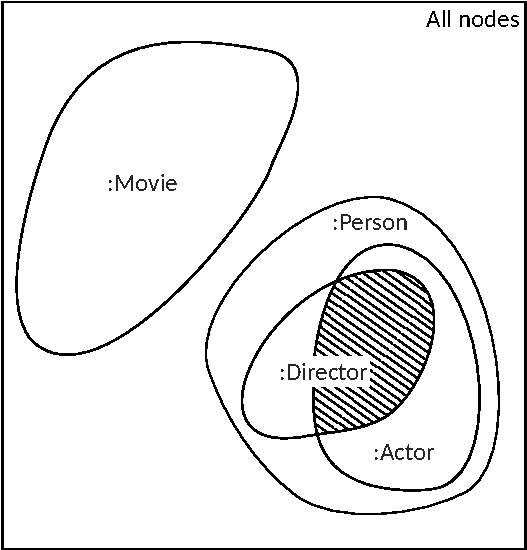
\includegraphics[width=0.4\textwidth]{figures/nodes-venn-diagram.pdf}
  \caption{Distribution of node labels in a example database.}
  \label{fig:label-dist-example}
\end{figure}

From this diagram, we can conclude that movies and persons are disjoint.
We also see that, persons, actors and directors do strongly overlap.
Consequently, the following label partition might be a good choice:
\[
  \lpart := \{ \{ \text{Movie} \},
               \{ \text{Person}, \text{Actor}, \text{Director} \} \}
\]

We highlight one option for a partition, which we call the
\emph{strict partition}. First, we define a relation for overlapping labels:
\begin{align}
\begin{split}
  &\overlap \subseteq \nlabels^2 \\
  &l_1 ~\overlap~ l_2 ~:\Leftrightarrow~
    \selection{v:l_1}(\selection{v:l_2}(\getnodes{v})) \not = \emptyset
\end{split}
\end{align}
$\overlap$ is reflexive and symmetric and the transitive closure
$\overlap^+$ is thus an equivalence relation.

The strict partition $\strictlpart$ is simply the set of equivalence classes
of $\overlap^+$ (also called the quotient set):
\begin{align}
\begin{split}
  \strictlpart &:= \nlabels / \overlap^+ \\
               &= \{ \{ l' \in \nlabels \mid l ~\overlap^+~ l' \}
                      \mid l \in \nlabels \}
\end{split}
\end{align}

We observe that labels from different equivalence classes are disjoint:
Take two labels $l_1, l_2$ from different equivalence classes
$O_1, O_2 \in \strictlpart$. Then $(l_1, l_2) \not \in \overlap^+$.
This implies $(l_1, l_2) \not \in \overlap$ and therefore
$\selection{v:l_1}(\selection{v:l_2}(\getnodes{v})) = \emptyset$.
Note that the inverse is not necessarily true, there may be two labels in the
same equivalence class which are disjoint (this is a potential weakness of the
strict partition, see the remark below).

As a result, if $L \subseteq \nlabels$ contains two labels from different
members of $\strictlpart$ then $\prob{\Omega}(v{:}L) = 0$ for any query result
$\Omega$.

\begin{remark}
The strict partition can also be obtained using a single-linkage
hierarchical clustering that succesively merges all clusters of labels
having a cluster distance smaller than $1$ (using the Jaccard distance
measure defined in Equation \ref{eq:jacc-dist}).
Once the single-linkage algorithm has finished, two
labels from different clusters will have distance $1$, which means that their
node sets are disjoint.

Because the single-linkage algorithm tends to build long chains, it can happen
that many pairs of disjoint node labels end up in the same cluster.
This can be avoided by a different linkage criterion (e.g. average linkage).
\end{remark}

\subsection{Sublabel Map}
\label{sub:sublabel-map}

In addition to the partition, we generate a \emph{sublabel map} $\submap$.
The sublabel map assigns to each label all labels that are considered to be
sublabels of this label. Again, this map can be provided by the user or 
maintained by the DBMS.

In the example of Figure \ref{fig:label-dist-example}, a good sublabel map
would be
\begin{align*}
  &\submap(\text{Movie}) := \emptyset \\
  &\submap(\text{Person}) := \{ \text{Actor}, \text{Director} \} \\
  &\submap(\text{Actor}) := \emptyset \\
  &\submap(\text{Director}) := \emptyset
\end{align*}

We define the \emph{strict sublabel map} as
\begin{align}
\begin{split}
  &\strictsubmap ~:~ \nlabels \rightarrow \powSet{\nlabels} \\
  &\strictsubmap(l) :=  \{ l' \in \nlabels \mid l' \subseteq l \}
\end{split}
\end{align}
Following this definition, if $l' \in \strictsubmap(l)$, then it follows
logically for all query results $\Omega$ that
$\prob{\Omega}(v{:}l \isect v{:}l') = \prob{\Omega}(v{:}l')$.

\begin{remark}
Again, the condition for the assumption of a sublabel relationship can be
weakened if necessary.
A straightforward option is the following definition of the sublabel map
\[
  \submap(l) :=  \{ l' \in \nlabels \mid
    \frac{\card{\selection{v:l'}(\selection{v:l}(\getnodes{v}))}}
         {\card{\selection{v:l'}(\getnodes{v})}} \geq \epsilon \}
\]
which considers those labels $l'$ sublabels of $l$ whose nodes are contained in
the nodes of $l$ to a (tunable) degree $\epsilon$.
\end{remark}

\section{Solving the Problem of Global Assumptions}
\sectionmark{Solution}

We will now show how to address the problem of global assumptions using a label
partition $\lpart$ and a sublabel map $\submap$.

Suppose a set $L \subseteq \nlabels$ of node labels.

If there are two node labels $l_1, l_2 \in L$ with
$\lpart(l_1) \not = \lpart(l_2)$, then the label partition tells us we should
assume $\prob{\getnodes{v}}(v{:}l_1 \isect v{:}l_2) = 0$. This implies
$\prob{\Omega}(v{:}l_1 \isect v{:}l_2) = 0$ and therefore
\[
  \prob{\Omega}(v{:}L) \approx 0 ~\text{.}
\]

On the contrary, if all labels from $L$ are in the same member set of $\lpart$,
we make use of the sublabel map to simplify the probability expression.
Take a label $l \in L$. If $s(l) \isect L \not = \emptyset$ then the sublabel
map tells us to assume that $L$ contains a sublabel $l' \subseteq l$.
This means that
$\prob{\getnodes{v}}(v{:}l' \isect v{:}l) \approx \prob{\getnodes{v}}(v{:}l')$
and implies
$\prob{\Omega}(v{:}l' \isect v{:}l) \approx \prob{\Omega}(v{:}l')$.

Iterative application of this simplification gives us a smaller set of labels
$L' := \{ l \in L \mid s(l) \isect L = \emptyset \}$, with
\[
  \prob{\Omega}(v{:}L) \approx \prob{\Omega}(v{:}L') ~\text{.}
\]

Now we are left with a set of labels $L'$, which contains overlapping labels
that are not sublabels of each other.
We do now finally assume these labels are independent in $\Omega$, which
gives us the solution
\[
  \prob{\Omega}(v{:}L) \approx \prod_{l \in L \land s(l) \isect L = \emptyset}
                                 \prob{\Omega}(v{:}l)
\]

All in all, we can compute the probability of drawing a subgraph where the
nodes matched by $v$ have the labels $L$ as
\begin{align}
  \prob{\Omega}(v{:}L) \approx
                         \begin{cases}
                           0, \text{ if there are } l_1, l_2 \in L
                              \text{ such that } D(l_1) \not = D(l_2) \\
                           \prod_{l \in L \land s(l) \isect L = \emptyset}
                             \prob{\Omega}(v{:}l), \text{ otherwise}
                         \end{cases}
\end{align}

For instance, in the example of Figure \ref{fig:label-dist-example}, using the
proposed label partition and sublabel map, we have
\begin{align*}
  \prob{\Omega}(v{:}\text{Person} \isect v{:}\text{Actor}
                \isect v{:}\text{Director})
    &\approx \prob{\Omega}(v{:}\text{Actor})
             \cdot \prob{\Omega}(v{:}\text{Director})
\end{align*}
\[
  \prob{\Omega}(v{:}\text{Director} \isect v{:}\text{Movie}) \approx 0
\]


\chapter{Logical Properties}
\label{chap:log-props-framework}

\begin{aboutchapter}
In Chapter \ref{chap:query-algebra} we have given a formal definition of a
graph database and a suitable query algebra.
In this Chapter, we explain the Cascades framework for the estimation
of so-called logical properties of query results. The result cardinality
appears in this framework as one particular logical property.
\end{aboutchapter}

\section{Logical vs. Physical Properties}

According to Graefe\cite{graefe_volcano_1993}, data can have logical and
physical properties.
Logical properties are properties that can be logically deduced from the data,
whereas physical properties depend on the physical
environment in which the data is processed.

\paragraph{Logical Database Properties}
\label{def:log-database-props}
  
A logical database property is simply a function of the database graph $G$.
We are often interested in functions with some numerical output, e.g. the
number of nodes, average density etc.
Every DBMS maintains a set of logical database properties which can be used
by the query optimizer to estimate result cardinalities.

We write $\props{G}$ to refer to the logical database properties, that are
maintained by a particular DBMS with database graph $G$.

\paragraph{Logical Result Properties}
\label{def:log-result-props}
  
A logical result property is simply a function of a query result.
The most important logical result property in query optimization is the
result cardinality.

We write $\props{\Omega}$ to refer to the set of logical result properties
used in a particular DBMS for a query result $\Omega$.

\section{Estimating Logical Result Properties of Operator Trees}
\sectionmark{Estimation}

In our graph database model, queries can be expressed as a tree of algebra operators.
During query optimization, we want to estimate the result cardinality
of such a tree. This estimation has to be done before the query is executed and
should be very fast.

In Cascades, the problem of cardinality estimation is decomposed into
subproblems, corresponding to the operators in the tree.

The structure of such a subproblem is shown in Figure \ref{fig:op-dependencies}.
Each operator has a finite number of inputs, which determine the result.
Suppose that we know a set of logical properties of each input of an operator.
Then we can use this information to estimate the logical properties of the
result, including the result cardinality.

\begin{figure}[h]
  \centering
  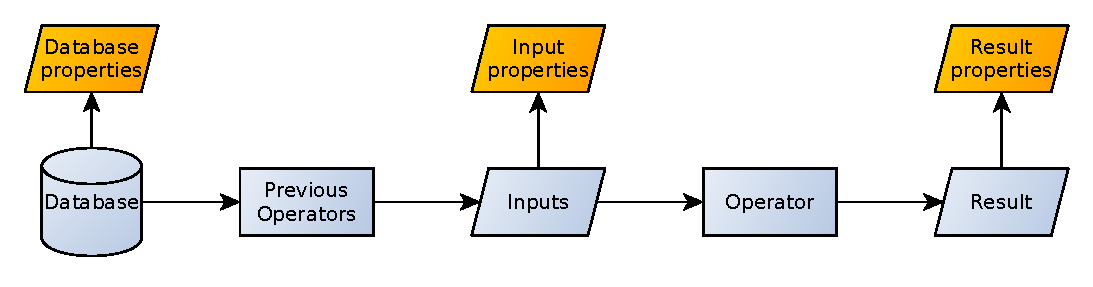
\includegraphics[width=0.9\textwidth]{figures/operator_properties_dependencies.pdf}
  \caption{Dependencies between operator inputs, result and logical
           properties.}
  \label{fig:op-dependencies}
\end{figure}

The estimated result properties can then be used as the input properties in the
next estimation step. The resulting chain of estimations is shown in
Figure \ref{fig:prop-estimation}.

\begin{figure}[h]
  \centering
  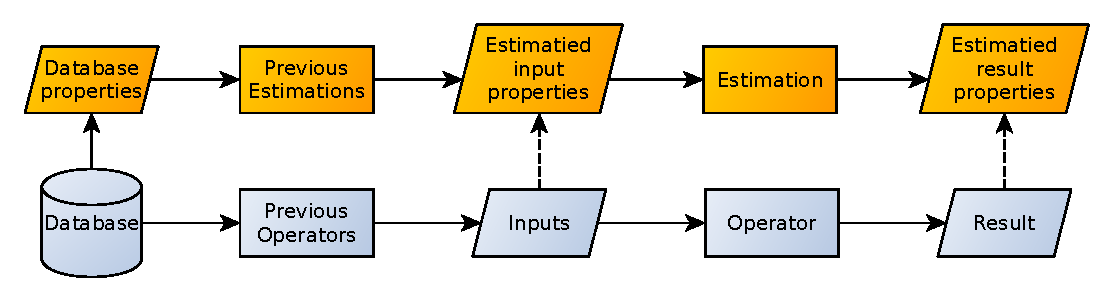
\includegraphics[width=0.9\textwidth]{figures/properties_estimation.pdf}
  \caption{Estimation of result properties.}
  \label{fig:prop-estimation}
\end{figure}


The more information we put into the logical properties, the more precise the
estimations will be. If the information is insufficient, the estimations can
diverge from the actual logical properties in a longer estimation chain
(symbolized by the dashed arrows in the above Figure).
However, storing more information also means increasing
memory consumption and processing time. This tradeoff has to be optimized.

In the following definitions, we formalize the idea that was just presented.

\begin{definition}[Estimation function]
  $\estfunc{o}$ is a logical properties estimation function of the operator
  $o \in \operators$ iff it has the following signature:\\
  
  \begin{samepage}
  \textbf{Input:}
  \begin{enumerate}
    \item $\props{G}$, the logical database properties.
    \item $\estprops{i_1}, \ldots, \estprops{i_n}$,
      the estimated logical properties of all inputs $i_1, \ldots, i_n$ of $o$.
  \end{enumerate}
  
  \textbf{Output:}\\
  
  $\estprops{o(i_1, \ldots, i_n)}$, an estimation of the logical properties of the
  output.
  \end{samepage}
\end{definition}

\begin{definition}[Estimated logical properties of an operator tree.]
  We define the estimated logical properties $\estprops{\Omega}$ of an
  operator tree $\Omega = o(i_1, \ldots, i_n)$ as
  \begin{displaymath}
    \estprops{\Omega}
      := \estfunc{o}(\props{G}, \estprops{i_1}, \ldots, \estprops{i_n})
  \end{displaymath}
\end{definition}

Now the logical properties of an operator tree can be estimated recursively as
shown in Figure \ref{fig:estimation-tree}.

\begin{figure}[ht]
 \begin{center}
   \begin{tikzpicture}
    \newcommand{\E}[1]{\estfunc{#1}}
    \small
    
    \node [block] (query) {
      $\estprops{\selection{h : \{ \text{Hobby} \}}(\expandout{x}{l : \{ \text{LIKES} \}}{h}(\selection{x : \{ \text{Person} \}}(\getnodes{x})))}$
    };
    
    \node [block] (hobby-label-selection) [below = of query] {$\E{\selection{h : \{ \text{Hobby} \}}}$};
    \node [block] (likes-expand) [below = of hobby-label-selection] {$\E{\expandout{x}{l : \{ \text{LIKES} \}}{h}}$};
    \node [block] (person-label-selection) [below = of likes-expand] {$\E{\selection{x : \{ \text{Person} \}}}$};
    \node [block] (get-nodes-as-x) [below = of person-label-selection] {$\E{\getnodes{x}}$};
    
    \draw[->] (likes-expand) edge node {} (hobby-label-selection);
    \draw[->] (person-label-selection) edge node {} (likes-expand);
    \draw[->] (get-nodes-as-x) edge node {} (person-label-selection);
    
    \node [block] at ([xshift=2cm]get-nodes-as-x.center) (db-props) {$\props{G}$};
    \draw[->] ([xshift=2cm]hobby-label-selection.center) -- (hobby-label-selection);
    \draw[->] ([xshift=2cm]likes-expand.center) -- (likes-expand);
    \draw[->] ([xshift=2cm]person-label-selection.center) --  (person-label-selection);
    \draw[->] (db-props) -- (get-nodes-as-x);
    \draw[-] (db-props) -- ([xshift=2cm]hobby-label-selection.center);
    
    \draw ([xshift=-0.5mm]hobby-label-selection.north) -- ([xshift=-0.5mm]query.south);
    \draw ([xshift=0.5mm]hobby-label-selection.north) -- ([xshift=0.5mm]query.south);
\end{tikzpicture}

 \end{center}
 \caption{Estimation graph for the logical properties of an operator tree.}
 \label{fig:estimation-tree}
\end{figure}

We will use these Definitions in our Neo4j implementation
(see Chapter \ref{chap:neo4j-impl}).


\chapter{Cardinality Estimation Model}
\chaptermark{Estimation Model}

\label{chap:neo4j-impl}

\begin{aboutchapter}
In this chapter, we use the query algebra defined
in Chapter \ref{chap:query-algebra} and the logical properties framework
defined in Chapter \ref{chap:log-props-framework}
to implement cardinality estimations for Neo4j.
Our estimations use a label partition and a sublabel map (cf. Section
\ref{sec:more-label-info}) as additional
information to the Neo4j statistics.
\end{aboutchapter}

\section{The Neo4j Graph Database}
\label{sec:about-neo4j}

Neo4j\footnote{\url{https://neo4j.com/}}
is a popular graph database written in Java. In Neo4j, a database consists of a
\emph{property graph}. A property graph is an extension of a labeled and typed
multigraph (cf. Definition \ref{def:database-graph}) that allows to store
properties at nodes.
Key to Neo4j's popularity is the expressive and user-friendly query language
\emph{Cypher}.

Our query algebra can be used to express an important subset of Cypher, namely
the matching of subgraphs with label, type and uniqueness constraints.

Because Neo4j is open-source software and thus easy to modify, we use
it as testbed for our cardinality estimations.

\section{Query Language Restrictions}
\label{sec:query-restrictions}

Due to three limitations, we can only provide estimations for a restricted
query space.

Firstly, the estimations developed in this thesis are tested in the JCascades
framework.
JCascades is a general Java implementation of the Cascades
framework for query optimization and is developed at the University of
Konstanz. In its current state of development it lacks support for certain
kinds of operators, including the \op{NodeJoin} operator.

Secondly, to estimate the result cardinalities of cyclic queries
(i.e., subgraph patterns containing a cycle), we
need statistics about the likeliness of cycles in the database.
Unfortunately, Neo4j currently lacks such statistics.
Implementing these statistics is not possible as part of this
work, due to limited resources and time.
Therefore we do not consider cyclic queries, i.e. queries containing
a \op{Traverse} operator.

Thirdly, in this first version of the estimations, we do not cover the
\op{DistinctSelection} operator. This is for time reasons only.

As a result, our estimations only cover the incomplete set of operators
\[
  \{ \getnodes{v}, \selection{v:l},
     \expandvar{v}{r:T}{\alpha}{w} \}
\]

The fraction of the result space covered by these operators consists of all
query results produced by non-cyclic subgraph patterns having only one
single component and no uniqueness constraints.
That is, all query results produced by \emph{tree subgraph patterns} with no
uniqueness constraints.
In Section \ref{sec:cypher-to-operators} we define the corresponding subset of
Cypher.

\section{Logical Database Properties}
\label{sec:logical-database-props}

The estimations developed in this thesis are intended to be usable in the Neo4j
graph database. Therefore, the logical database properties used in the
estimations are very similar to those available in the Neo4j statistics.

For convenience we use $*$ as a wildcard label that selects all nodes and
similarly as a wildcard relationship type that allows all relationship types.
Let $l, l_1, l_2 \in \nlabels \cup \{ * \}, t \in \rtypes \cup \{ * \}$ and
$\alpha \in \{\leftarrow, \rightarrow \}$.
The wildcard label selection is defined as $\selection{v:*}(\Omega) := \Omega$.

We require the following logical database properties $\props{G}$.
\begin{enumerate}[1.]
  \item The number of nodes in $G$ having the label $l$.
    \[
      N(l) := \card{\selection{v:l}(\getnodes{v})}
    \]
  \item The number of outgoing/incoming relationships of type $t$ in $G$
    from nodes with label $l_1$ to nodes with label $l_2$ (sometimes called
    triple statistics).
    \[
      R_\alpha(l_1, t, l_2) := \card{\selection{w:l_2}(
        \expandvar{v}{r:T}{\alpha}{w}(\selection{v:l_1}(\getnodes{v}))
        )}
    \]
    where $T := \begin{cases}
                  \rtypes \text{ if } t = *, \\
                  \{ t \}, \text{ otherwise}
                \end{cases}$.
  \item A label partition $\lpart$ as described in Section
    \ref{sub:label-partition}.
  \item A sublabel map $\submap$ as described in Section
    \ref{sub:sublabel-map}.
\end{enumerate}

Neo4j offers all of these logical database properties, but it estimates
\[
  R_\alpha(l_1, t, l_2) \approx \min \{ R_\alpha(l_1, t, *),
                                        R_\alpha(*, t, l_2) \}
\]
Our estimations require the actual values of $R_\alpha(l_1, t, l_2)$
to yield good results. Hence, we have to implement the collection of these
values. Currently this is done by executing the corresponding queries
in Neo4j and storing the result cardinalities in a CSV file.
In the future, this should be integrated into the Neo4j statistics and updated
online.

Because every relationship has exactly one type, we can obtain the number of
relationships of any type in $T \subseteq \rtypes$ and any direction $\alpha$
between nodes with label $l_1$ to nodes with label $l_2$ as
\[
  R_\alpha(l_1, T, l_2) = \sum_{t \in T} R_\alpha(l_1, t, l_2)
\]

Furthermore, we can define the average degree in $\alpha$ direction as
\[
  \avgdeg_\alpha(l_1, T, l_2) := \frac{R_\alpha(l_1, T, l_2)}{N(l_1)}
\]

\section{Logical Result Properties}
\label{sub:neo4j-log-result-props}

As described in Chapter \ref{chap:log-props-framework} the logical properties of
a query result $\Omega$ are estimated by building a chain of estimation
functions.
If the information content of the logical result properties is too small,
it can happen that the estimated properties diverge from reality for
queries incorporating many operators.

To limit this risk, we store a subgraph pattern $\rho(\Omega)$ producing the
query result in the logical properties (in Section \ref{sec:completeness} we
have shown that such a subgraph pattern exists for all query results).
From this pattern, the estimation functions know about all the previous
operators in the estimation chain.

In addition, we store for all node variables $v \in \nvars(\Omega)$ the
probability of drawing a subgraph from the query result where the node matched
by $v$ has the label $l$, $\prob{\Omega}(v{:}l)$
(cf. Equation \ref{eq:label-probability}).

We also store a Boolean flag, indicating whether the result was produced by the
\op{GetNodes} operator:
\begin{align}
  \initial(\Omega) :\Leftrightarrow \Omega = \getnodes{v}
    \text{ for some } v \in \qvars
\end{align}

Finally, the logical result properties contain the result cardinality
$\card{\Omega}$.
The memory requirements of the logical properties are shown in Table
\ref{table:neo4j-log-result-props-mem-reqs}.

\begin{table}[H]
\centering
\begin{tabular}{ll}
\toprule
Component                  & Space complexity                                                     \\ \midrule
Subgraph pattern           & $O(\binom{\card{R_\rho}}{2} + \card{V_\rho} \cdot \card{\nlabels})$
                             (cf. Table \ref{table:subgraph-pattern-mem-reqs})                    \\[3pt]
Label probabilities        & $O(\card{V_\rho} \cdot \card{\nlabels})$                             \\[3pt]
Initial flag               & $O(1)$                                                               \\[3pt]
Result cardinality         & $O(1)$                                                               \\[3pt]
\textbf{Total:}            & $O(\binom{\card{R_\rho}}{2}) + \card{V_\rho} \cdot \card{\nlabels})$ \\
\bottomrule
\end{tabular}
\caption{Space complexity of the logical result properties.}
\label{table:neo4j-log-result-props-mem-reqs}
\end{table}

\begin{remark}
From a purely logical perspective, the label probabilities, the initial flag
and the result cardinality are already determined by the subgraph pattern.

However, the logical result properties are not intended to be logically
minimal, but to allow for \emph{efficient} computations in the estimation
functions.

Deducing the exact cardinality from the subgraph pattern would often
require to execute the query, which we want to avoid.
Instead, we want a \emph{fast estimation} of the output cardinality,
which is only possible if we store logically redundant information.
\end{remark}

%TODO: rethink title
\section{Assumption About Node Degrees}
\sectionmark{Degree Assumption}

We assume node degrees are approximately uniformly distributed among
nodes with the same label, i.e. the individual node degrees are close
enough to the average degree to use it as an estimation:
For any query result $\Omega$, node variables $x, y$ and relationship
directions $\alpha \in \{ \leftarrow, \rightarrow \}$ and for any node labels
$l_1 \in \nlabels, l_2 \in \nlabels \cup \{ * \}$ we have:
\begin{align}
  \card{\selection{y:l_2}(\expandvar{x}{r:T}{\alpha}{y}(
                       \selection{x:l_1}(\Omega)
                     ))}
  \approx
    \card{\selection{x:l_1}(\Omega)} \cdot \avgdeg_\alpha(l_1, T, l_2)
  \label{ass:uniformity-1}
\end{align}

For nodes not having any label, we assume the node degree equals the overall
average node degree:
\begin{align}
  \card{\selection{y:l_2}(\expandvar{x}{r:T}{\alpha}{y}(
     \Omega \setminus \bigunion_{l_1 \in \nlabels} \selection{x:l_1}(\Omega)
  ))}
  \approx
    \card{\Omega \setminus
      \bigunion_{l_1 \in \nlabels} \selection{x:l_1}(\Omega)}
    \cdot \avgdeg_\alpha(*, T, l_2)
  \label{ass:uniformity-2}
\end{align}

\section{Estimation Functions}

An estimation function for the logical result properties of an operator $o$
takes a subgraph pattern, an initial flag, label probabilities and a cardinality
corresponding to the input and computes a new subgraph pattern, a new initial
flag, new label probabilities and a new result cardinality corresponding to the
result of $o$ (see Section \ref{sub:neo4j-log-result-props}).

We have to define such an estimation function for every operator of our
query algebra.

From the proofs that the individual operators are well-defined, we already
know how to compute the result subgraph pattern from the input subgraph
pattern for every operator (cf. Section \ref{sec:operators}).
Therefore, we only have to define functions for the initial flag, the result
cardinality and the label probabilities.

\subsection{Estimation for \op{GetNodes}}
$\getnodes{v}$ returns the set of all single node subgraphs of $G$,
matched by the variable $v$.

\paragraph{Initial flag}

The result is initial:
\begin{align}
  \initial(\getnodes{v}) \Leftrightarrow \true
\end{align}

\paragraph{Result cardinality}

The result cardinality is the number of nodes in the database:
\begin{align}
  \card{\getnodes{v}} = N(*)
\end{align}

\paragraph{Label probabilities}

The probability of drawing a node matched by $v$, having a particular label $l$
equals the fraction of nodes in the database having this label: 
\begin{align}
\begin{split}
  \prob{\getnodes{v}}(v{:}l) &= \frac{\card{\selection{v:l}(\getnodes{v})}}
                                     {\card{\getnodes{v}}} \\
                             &= \frac{N(l)}{N(*)}
\end{split}
\end{align}


\subsection{Estimation for \op{NodeLabelSelection}}

$\selection{v:l}(\Omega)$ keeps all subgraphs from $\Omega$, where the node
matched by $v$ has the label $l$.

\paragraph{Initial flag}

The result of the selection is initial, iff the input is initial and all
nodes matched by $v$ in the input have the label $l$:
\begin{align}
\begin{split}
  \initial(\selection{v:l}(\Omega))
    &\Leftrightarrow \selection{v:l}(\Omega) = \getnodes{v} \\
    &\Leftrightarrow \Omega = \getnodes{v} \land
      \frac{\card{\selection{v:l}(\getnodes{v})}}
           {\card{\getnodes{v}}} = 1 \\
    &\Leftrightarrow \initial(\Omega) \land
      \prob{\Omega}(x{:}l) = 1
\end{split}
\end{align}

\paragraph{Result cardinality}

The result cardinality of the selection is given as:
\begin{align}
\begin{split}
  \card{\selection{v:l}(\Omega)} &= \frac{\card{\selection{v:l}(\Omega)}}
                                         {\card{\Omega}}
                                    \cdot \card{\Omega} \\
                                 &= \prob{\Omega}(v{:}l) \cdot \card{\Omega}
\end{split}
\end{align}

\paragraph{Label probabilities}

We derive the new label probabilities using a case distinction.

We first look at the label probabilities at the variable $v$.
Firstly, in the result all nodes matched by $v$ have the label $l$:
\begin{align}
\begin{split}
  \prob{\selection{v:l}(\Omega)}(v{:}l)
    &= \frac{\card{\selection{v:l}(\selection{v:l}(\Omega))}}
            {\card{\selection{v:l}(\Omega)}} \\
    &= \frac{\card{\selection{v:l}(\Omega)}}
            {\card{\selection{v:l}(\Omega)}} \\
    &= 1
\end{split}
\end{align}
The same holds for all nodes matched by $v$ having a superlabel of $l$, i.e.,
$\prob{\selection{v:l}(\Omega)}(v{:}l') = 1$ if $l \in \submap(l')$.

Now take a label $l' \in \nlabels, l' \not = l$. If
$\lpart(l') \not = \lpart(l)$, then we assume the labels are disjoint and we
have
\begin{align}
\begin{split}
  \prob{\selection{v:l}(\Omega)}(v{:}l')
    &= \frac{\card{\selection{v:l'}(\selection{v:l}(\Omega))}}{\card{\selection{v:l}(\Omega)}} \\
    &= \frac{\prob{\Omega}(v{:}l' \isect v{:}l)}{\prob{\Omega}(v{:}l)} \\
    &\approx 0
\end{split}
\end{align}

Else, if $l' \in s(l)$, then we assume that $l'$ is a sublabel of $l$:
\begin{align}
\begin{split}
  \prob{\selection{v:l}(\Omega)}(v{:}l')
    &= \frac{\prob{\Omega}(v{:}l' \isect v{:}l)}{\prob{\Omega}(v{:}l)} \\
    &\approx \frac{\prob{\Omega}(v{:}l')}{\prob{\Omega}(v{:}l)}
\end{split}
\end{align}

Else, we assume that $l$ and $l'$ are independent in $\Omega$:
\begin{align}
\begin{split}
  \prob{\selection{v:l}(\Omega)}(v{:}l')
    &= \frac{\prob{\Omega}(v{:}l' \isect v{:}l)}{\prob{\Omega}(v{:}l)} \\
    &\approx \frac{\prob{\Omega}(v{:}l') \cdot \prob{\Omega}(v{:}l)}{\prob{\Omega}(v{:}l)} \\
    &= \prob{\Omega}(v{:}l')
\end{split}
\end{align}

Now take a node variable $v'$ with $v' \not = v$.
The problem is to compute the expression
\begin{align}
\begin{split}
  \prob{\selection{v:l}(\Omega)}(v'{:}l')
    &= \frac{\prob{\Omega}(v'{:}l' \isect v{:}l)}{\prob{\Omega}(v{:}l)} \\
\end{split}
\end{align}
This is impossible without exploiting information about how $v$ and
$v'$ are connected in the subgraph pattern $\rho$.
Although we have this information available from $\rho$ in theory, using it
would require potentially costly traversals of the pattern and significantly
increase the amount of time required to compute the new label probabilities.

Instead, we assume that the events $v'{:}l'$ and $v{:}l$ are independent in
$\Omega$, i.e., that selecting a label on one node variable of a pattern does
not affect the distribution of labels at other node variables of this pattern:
\begin{align}
\begin{split}
  \prob{\selection{v:l}(\Omega)}(v'{:}l') \approx \prob{\Omega}(v'{:}l')
\end{split}
\end{align}

\begin{remark}
This assumption somehow contradicts the motivation of the thesis, because it
neglects the possibility of strong correlations between the existence of
relationships between nodes and the labels of these nodes.

In future revisions of this work another solution might be proposed.
However, the current assumption allows for very local updates to the
label probabilities (only the probabilities at the variable $v$ must be
updated) and can therefore be computed very fast.

Also note that, correlations between relationship types and labels are
considered in the estimation functions of the \op{Expand} operator.
\end{remark}

\subsection{Estimation for \op{Expand}}

$\expandvar{x}{r:T}{\alpha}{y}(\Omega)$ expands the subgraphs in $\Omega$
by matching relationships $r$ of types $T$ starting at nodes matched by $x$
and going to nodes matched by $y$ in direction $\alpha$.

\paragraph{Initial flag}

The result of an expand is never initial:
\begin{align*}
  \initial(\expandvar{x}{r:T}{\alpha}{y}(\Omega))
    &\Leftrightarrow \expandvar{x}{r:T}{\alpha}{y}(\Omega) = \getnodes{x} \\
    &\Rightarrow \rvars(\expandvar{x}{r:T}{\alpha}{y}(\Omega))
                 = \rvars(\getnodes{x}) \\
    &\Rightarrow \{ r \} \subseteq \emptyset \\
    &\Leftrightarrow \false
\end{align*}

\paragraph{Result cardinality}

If the input $\Omega$ is initial, i.e. it is the result of a \op{GetNodes}
operator, we know the exact result cardinality from the database properties:
\begin{align}
  \card{\expandvar{x}{r:T}{\alpha}{y}(\getnodes{x})} = R_\alpha(*, T, *)
\end{align}

Let us now focus on the case where $\Omega$ is not initial.
The idea of the estimation function for the result cardinality is to
describe the nodes matched by the variable $v$ in $\Omega$
in terms of their node labels.

Because there is only a finite number of labels in the database, we can
enumerate them according to the partition of overlapping labels:
Let $\lpart_i$ be the $i$-th member set of $\lpart$ and
$l_{i,j}$ the $j$-th label in $\lpart_i$.

For each node, \emph{one} node label $l$ is chosen that is considered to be
most representative for this node.
The degree of the node is then estimated as the average degree
$\avgdeg_\alpha(l, T, *)$ of all nodes having this representative label.
The assignment of nodes to representative labels happens using the information
stored in the input label probabilities, the label partition $\lpart$ and the
sublabel map $\submap$.

\vspace{1em}
In the first step, we divide the set of input subgraphs into two subsets.
In the first subset, we put those subgraphs where the nodes matched by $x$
have any label. In the second subset, we put the subgraphs where the nodes
matched by $x$ have no label:
\begin{align}
\begin{split}
  \card{\expandvar{x}{r:T}{\alpha}{y}(\Omega)}
               = &\card{\expandvar{x}{r:T}{\alpha}{y}(
                    \bigunion_{l \in \nlabels} \selection{x:l}(\Omega))}
                      ~~\text{(1)} \\
                   &+ \\
                   &\card{\expandvar{x}{r:T}{\alpha}{y}(
                     \Omega \setminus
                       \bigunion_{l \in \nlabels} \selection{x:l}(\Omega))}
                         ~~\text{(2)}
\end{split}
\end{align}

We now rewrite the first term as a sum over the member sets of the node label
partition $\lpart$. After that, we add an inner sum over the
respective node labels of each member set.
For each node label $l_{i,j} \in \lpart_i$, we count the
number of subgraphs produced by the expand applied on the nodes in $\Omega$
which have the label $l_{i,j}$, but do not have any of the labels
$l_{i,1}, \ldots, l_{i, j-1}$.
These nodes are then considered to be best represented by the label $l_{i,j}$.
Therefore, their degree is estimated as $\avgdeg_\alpha(l_{i,j}, T, *)$, using
the degree uniformity assumption. This gives us the following result:
\begin{align}
\begin{split}
  \text{(1)} &= \card{\expandvar{x}{r:T}{\alpha}{y}(\bigunion_{l \in \nlabels} \selection{x:l}(\Omega))} \\
             &\approx \sum_{i=1}^\card{\lpart}
                  \card{\expandvar{x}{r:T}{\alpha}{y}(\bigunion_{j=1}^\card{\lpart_i}
                  \selection{x:l_{i,j}}(\Omega))} \\
             &= \sum_{i=1}^\card{\lpart}
                \sum_{j=1}^\card{\lpart_i}
                  \card{\expandvar{x}{r:T}{\alpha}{y}(\selection{x:l_{i,j}}(
                  \Omega \setminus \bigunion_{k=1}^{j-1} \selection{x:l_{i,k}}(\Omega)
                  ))} \\
            \text{\tiny Equation \ref{ass:uniformity-1}} &\omit\dotfill \\
             &\approx \sum_{i=1}^\card{\lpart}
                      \sum_{j=1}^\card{\lpart_i}
                        \card{\selection{x:l_{i,j}}(
                        \Omega \setminus \bigunion_{k=1}^{j-1} \selection{x:l_{i,k}}(\Omega)
                        )}
                        \cdot \avgdeg_\alpha(l_{i,j}, T, *) \\
             &= \sum_{i=1}^\card{\lpart}
                \sum_{j=1}^\card{\lpart_i}
                  \card{\Omega}
                  \cdot \prob{\Omega}(x{:}l_{i,j} \isect \overline{\bigunion_{k=1}^{j-1} x{:}l_{i,k}})
                  \cdot \avgdeg_\alpha(l_{i,j}, T, *) \\
             &= \card{\Omega}
                \cdot
                \sum_{i=1}^\card{\lpart}
                \sum_{j=1}^\card{\lpart_i}
                  \prob{\Omega}(x{:}l_{i,j} \isect \bigisect_{k=1}^{j-1} \overline{x{:}l_{i,k}})
                  \cdot \avgdeg_\alpha(l_{i,j}, T, *)
\end{split}
\end{align}

At this point, we want to highlight a strength of our approach:
By taking into account the label probabilities of the input, the estimations
are precise even if there are strong dependencies between labels and the
presence of relationships.
If e.g., the input consists only of nodes having exactly one particular label,
then only the average degree of nodes of this label is used to estimate the
result cardinality.
Neo4j does not track label probabilities and is therefore unable to deal with
such dependencies.

The remaining problem is to sensibly estimate
$\prob{\Omega}(x{:}l_{i,j} \isect
               \bigisect_{k=1}^{j-1} \overline{x{:}l_{i,k}})$, which is the
fraction of subgraphs in $\Omega$ where the nodes matched by $x$ have the label
$l_{i,j}$ but none of the labels $l_{i,1}, \ldots, l_{i,j-1}$.

We observe that, if a node has several labels, the representative label is the
one that comes first in the ordering in the member set of the label partition.
Consequently, this ordering plays an essential role in the quality of the
estimation function.

A simple approach is to sort the labels $l$ descendingly by the product
$\sprob(l) \cdot \frac{1}{N(l)}$. This puts the labels in front that cover
most of the nodes matched by $x$ in $\Omega$ and whose number
of nodes in the database is closest to $\Omega$. If this value is similar for
two different labels, the label $l$ with higher $\sprob(l)$ comes first in the
ordering.
We will use this ordering for the estimation function.

\begin{remark}
This simple approach does not take into account that nodes can be
matched several times by the same variable $x$ in different subgraphs of
$\selection{x:l}(\Omega)$.
It can happen that $x$ matches only one single node in the database in all
subgraphs of $\Omega$ while $\sprob(l) = 1$ and $N(l) = \card{\Omega}$.
In this case, the risk of an estimation error is very high, because it is
probable that this single node having label $l$ behaves differently than
a larger sample of nodes having $l$.

This problem could be addressed by sorting the labels according to a similarity
measure that describes the cardinality of the intersection of the nodes
matched by $x$ in $\selection{x:l}(\Omega)$ and in
$\selection{x:l}(\getnodes{x})$.
However, such a similarity measure would require storing and updating
information about the uniqueness of nodes matched by a particular node variable
and having a particular label.
\end{remark}

Now that we have discussed the ordering, we will present a solution for
computing
$\prob{\Omega}(x{:}l_{i,j}
       \isect \bigisect_{k=1}^{j-1} \overline{x{:}l_{i,k}})$.

To make the equations more readable, we write $\sprob$ for $\prob{\Omega}$.

Take a partition member set $\lpart_i \in \lpart$ and a subset of labels
$L \subset \lpart_i$. Take one label $l \in \lpart_i \setminus L$.

It holds that
\begin{align}
\begin{split}
  \sprob(l \isect \bigisect_{l' \in L} \overline{l'})
    &= \sprob(l \mid \bigisect_{l' \in L} \overline{l'})
       \cdot \sprob(\bigisect_{l' \in L} \overline{l'}) \\
    &= (1 - \sprob(\overline{l} \mid \bigisect_{l' \in L} \overline{l'}))
       \cdot \sprob(\bigisect_{l' \in L} \overline{l'}) \\
    &= (1 - \frac{\sprob(\bigisect_{l' \in L \union \{l\}} \overline{l'})}
                 {\sprob(\bigisect_{l' \in L} \overline{l'})})
       \cdot \sprob(\bigisect_{l' \in L} \overline{l'}) \\
    &= \sprob(\bigisect_{l' \in L} \overline{l'})
       - \sprob(\bigisect_{l' \in L \union \{l\}} \overline{l'})
    \label{eq:label-prob-1}
\end{split}
\end{align}

Take again a subset of labels $L \subset \lpart_i$ and a label
$l \in \lpart_i \setminus L$. For all $l' \in L$ that are sublabels
of $l$, the probability of drawing a node that does neither have the label
$l$ nor the label $l'$ equals the probability of drawing a node that does
not have the label $l$:
\begin{align*}
  \sprob(\overline{l} \isect \overline{l'}) \approx \sprob(\overline{l})
\end{align*}

Consequently, let $S := (L \setminus \submap(l)) \union \{l\}$. We have
\begin{align}
\begin{split}
  \sprob(\bigisect_{l' \in L \union \{l\}} \overline{l'})
    &\approx \sprob(\bigisect_{l' \in S \union \{l\}} \overline{l'})
    \label{eq:label-prob-2}
\end{split}
\end{align}

Iterative application of Equation \ref{eq:label-prob-2} gives us a minimal
set of superlabels $S^*$. For all $l \in S^*$, no sublabel of $l$ is contained
in $S^*$, i.e., $S^* \isect \submap(l) = \emptyset$.
For this set of superlabels we assume independence and obtain
\begin{align}
  \sprob(\bigisect_{l' \in S^*} \overline{l'})
    \approx \prod_{l' \in S^*} 1 - \sprob(l')
  \label{eq:label-prob-3}
\end{align}

Together, the Equations \ref{eq:label-prob-1} and \ref{eq:label-prob-3}
provide an easily computable, recursive estimation of
$\prob{\Omega}(x{:}l \isect \bigisect_{l' \in L} \overline{x{:}l'})$.


For the second term we apply the same technique:
\begin{align}
\begin{split}
  \text{(2)} &= \card{\expandvar{x}{r:T}{\alpha}{y}(
                      \Omega \setminus
                        \bigunion_{l \in \nlabels} \selection{x:l}(\Omega))} \\
            \text{\tiny Equation \ref{ass:uniformity-2}} &\omit\dotfill \\
             &\approx
                \card{\Omega \setminus
                        \bigunion_{l \in \nlabels} \selection{x:l}(\Omega)}
                \cdot \avgdeg_\alpha(*,T,*) \\
             &= \card{\Omega}
                \cdot \prob{\Omega}(\overline{\bigunion_{l \in \nlabels} x{:}l})
                \cdot \avgdeg_\alpha(*,T,*) \\
             &= \card{\Omega}
                \cdot (1 - \prob{\Omega}(\bigisect_{l \in \nlabels} x{:}l))
                \cdot \avgdeg_\alpha(*,T,*)
\end{split}
\end{align}

From Equation \ref{eq:label-prob-3} we know how to recursively compute the probability
expression in this formula.

\begingroup
\newcommand{\estDeg}{\textit{estDeg}}
\newcommand{\remaining}{\textit{remaining}}
\newcommand{\oldRemaining}{\textit{oldRemaining}}
\newcommand{\newRemaining}{\textit{newRemaining}}
\newcommand{\superLabels}{\textit{superLabels}}
\newcommand{\coveredLabels}{\textit{coveredLabels}}
\newcommand{\notCoveredBySuperLabels}{\textit{notCoveredBySuperLabels}}
\newcommand{\changed}{\textit{changed}}

To demonstrate the computability of the expand estimations,
we use Algorithm \ref{algo:expand-cardinality} that computes both terms (1)
and (2) in a single loop over the set of node labels.

The most interesting variables are the following:
\begin{itemize}
  \item $\estDeg$ stores the amount contributed to the total estimated degree
    by the nodes having one of the already covered labels ($\coveredLabels$).

  \item $\remaining$ stores the fraction of nodes matched by $v$ whose degree
    has not yet been estimated. After the loop has finished, this variable
    stores the fraction of nodes matched by $v$ not having any label, which
    allows to compute (2).

  \item $\superLabels$ stores the current minimal set of superlabels, as
    defined above. It is updated once in each iteration.

  \item $\notCoveredBySuperLabels$ stores the fraction of nodes matched by $v$
    that does not have any of these superlabels. If the minimal set of
    superlabels changes because of the current label, this variable has to be
    recomputed as a product over all superlabels.
    Otherwise, the cached value of the last iteration can be used and only a
    single multiplication is needed.
\end{itemize}

\begin{algorithm}
  \caption{{\sc computeExpandCardinality}}
  \label{algo:expand-cardinality}
  \DontPrintSemicolon
  \KwIn{$\estprops{\Omega}$ (estimation of the logical result properties of
        $\Omega$), $\props{G}$ (logical database properties)}
  \KwOut{estimation of $\card{\expandvar{x}{r:T}{\alpha}{y}(\Omega)}$}
  
  \eIf{$\initial(\Omega)$}{
      \tcp*[l]{We know the exact cardinality from the database properties.}
      \Return $R_\alpha(*, T, *)$\;
  }{
    \tcp*[l]{We estimate the cardinality by combining the node degrees for
             the different labels.}
    $\estDeg \gets 0$\;
    $\remaining \gets 1$\;
    
    \BlankLine
    \tcp*[l]{(1) Estimate the node degree for nodes having a label.}
    
    $i \gets 1$\;
    \While{$i < \card{\lpart} \land \remaining > 0$}{
      \tcp*[l]{Outer sum over the partition member sets.}
      
      $\oldRemaining \gets \remaining$\;
      $\superLabels \gets \emptyset$\;
      $\notCoveredBySuperLabels \gets 1$\;
      $\coveredLabels \gets \emptyset$\;
      
      $j \gets 1$\;
      \While{$j < \card{\lpart_i} \land \remaining > 0$}{
        \tcp*[l]{Inner sum over the labels in a partition member set.}
        
        \If{$l_{i,j} \not \in \coveredLabels$}{
          $\superLabels \gets (\superLabels \setminus \submap(l_{i,j}))$\;
          $\changed \gets \text{ whether } \superLabels \text{ has changed}$\;
          $\superLabels \gets \superLabels \union \{l_{i,j}\}$\;
          
          \eIf{$\changed$}{
            $\notCoveredBySuperLabels
              \gets \prod_{l \in \superLabels} 1 - \prob{\Omega}(x{:}l)$\;
          }{
            $\notCoveredBySuperLabels
              \gets \notCoveredBySuperLabels
                \cdot (1 - \prob{\Omega}(x{:}l_{i,j}))$\;
          }
        
          $\newRemaining \gets
            \notCoveredBySuperLabels - (1 - \oldRemaining)$\;
          
          $\estDeg \gets \estDeg + \avgdeg_\alpha(l_{i,j}, T, *)
            \cdot (\remaining - \newRemaining)$\;
          
          $\remaining \gets \newRemaining$\;
        }
        $\coveredLabels \gets \coveredLabels \union \submap(l_{i,j})$\;
        
        $j \gets j + 1$\;
      }
      $i \gets i + 1$\;
    }
    
    \BlankLine
    \tcp*[l]{(2) Estimate the node degree for nodes having no label.}
    
    $\estDeg \gets \estDeg + \avgdeg_\alpha(*, T, *) \cdot \remaining$\;
    
    \BlankLine
    \tcp*[l]{Compute the result cardinality.}
    
    \Return $\card{\Omega} \cdot \estDeg$\;
  }
\end{algorithm}

To better understand this algorithm, recall the example database about movies
and its distribution of node labels shown in Figure
\ref{fig:label-dist-example}.

In Figure \ref{fig:label-dist-example-with-result} we add to this diagram the
set of nodes matched by the variable $v$ of some query result $\Omega$.
Note that the size of the area does not necessarily
correspond to the cardinality of $\Omega$, as nodes can be matched several
times by the same variable in different subgraphs.

\begin{figure}
  \centering
  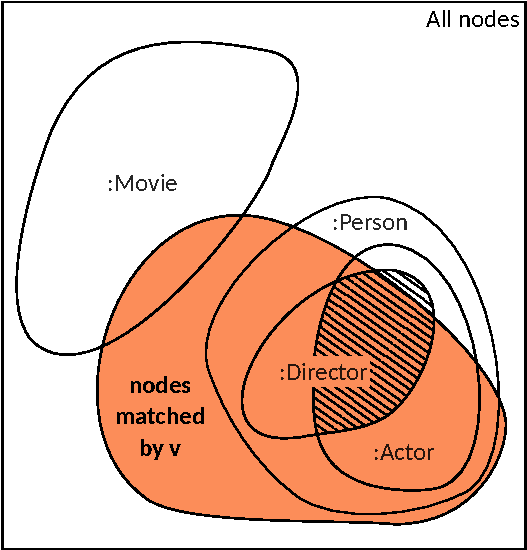
\includegraphics[width=0.4\textwidth]{figures/nodes-venn-diagram-with-query-result.pdf}
  \caption{Distribution of node labels and a query result in a example
           database.}
  \label{fig:label-dist-example-with-result}
\end{figure}

The outer loop of the algorithm iterates over the member sets of the label
partition. The inner loop iterates over the labels of one member set.
The order is given by the indices of the label variable $l_{i,j}$.
Suppose the algorithm iterates over the label partition in the following
order:
\begin{align*}
  l_{1,1} = \text{Movie} \\
  l_{2,1} = \text{Actor} \\
  l_{2,2} = \text{Director} \\
  l_{2,3} = \text{Person}
\end{align*}

We write again $\sprob(l)$ instead of $\prob{\Omega}(v{:}l)$ for better
readability.
The trace of the algorithm execution of the example is given by Table
\ref{table:expand-cardinality-trace-1} and Table
\ref{table:expand-cardinality-trace-2}.
Reading the tables from top to bottom we can see all variable assignments
performed by the algorithm in chronological order.
The column $l_{i,j}$ shows, which label is currently used to estimate the
degree of a fraction of the matched nodes.

Figure \ref{fig:expand-cardinality-steps} shows the usage of representative
labels for the nodes matched by $v$ as a sequence of Venn diagrams.
In each diagram, the orange area represents the fraction of nodes whose degree
is estimated in the current iteration of the algorithm.
The result of this estimation is written below the diagram (cf. the trace
of the algorithm in Table \ref{table:expand-cardinality-trace-1} and
Table \ref{table:expand-cardinality-trace-2}).
The total estimated degree of the nodes matched by $v$ is the sum of all the
partial degrees shown in the individual diagrams.

\begin{figure}
  \centering
  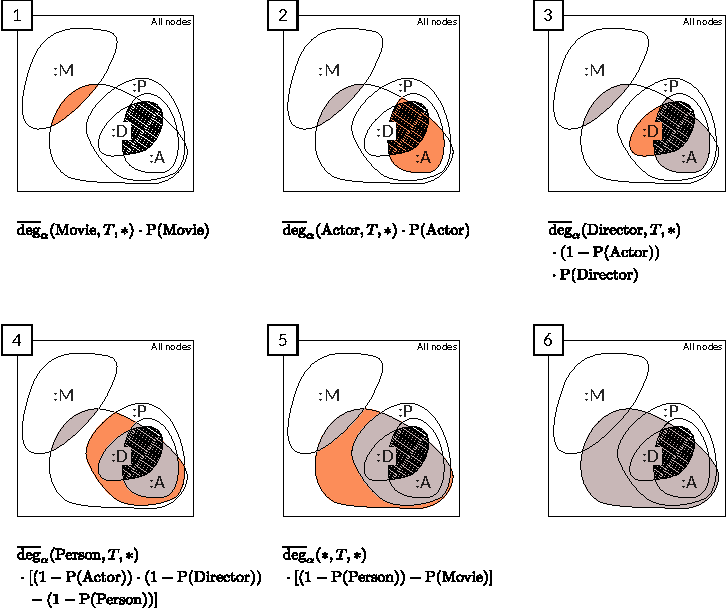
\includegraphics[width=\textwidth]{figures/labels-for-estimation-step-by-step-complete-formulas.pdf}
  \caption{Step-by-step visualization of the expand cardinality estimation.
           \textit{Orange:} The fraction of nodes whose degree is currently estimated.
           \textit{Grey:} Already covered fraction of nodes.
           \textit{Below each diagram:} The estimated degree corresponding to the orange fraction.}
  \label{fig:expand-cardinality-steps}
\end{figure}

\begin{landscape}
  \begin{table}[]
\vspace{-\marginparsep}
\vspace{-\marginparwidth}

\centering
\caption{Trace of the \textsc{ComputeExpandCardinality} algorithm (1).}
\label{table:expand-cardinality-trace-1}

\resizebox{\columnwidth}{!}{%
\begin{tabular}{lllllllllll}
$i$                       & $j$                       & $l_{i,j}$         & \estDeg                                                                  & \remaining                                                             & \oldRemaining             & \superLabels                                                & \coveredLabels                                                             & \notCoveredBySuperLabels                                                  & \changed                        & \newRemaining                                                          \\
                          &                           &                   & \cellcolor[HTML]{FC8D59}$0$                                              &                                                                        &                           &                                                             &                                                                            &                                                                           &                                 &                                                                        \\
                          &                           &                   &                                                                          & \cellcolor[HTML]{FC8D59}$1$                                            &                           &                                                             &                                                                            &                                                                           &                                 &                                                                        \\
\cellcolor[HTML]{FC8D59}1 &                           &                   &                                                                          &                                                                        &                           &                                                             &                                                                            &                                                                           &                                 &                                                                        \\
                          &                           &                   &                                                                          &                                                                        & \cellcolor[HTML]{FC8D59}1 &                                                             &                                                                            &                                                                           &                                 &                                                                        \\
                          &                           &                   &                                                                          &                                                                        &                           & \cellcolor[HTML]{FC8D59}$\emptyset$                         &                                                                            &                                                                           &                                 &                                                                        \\
                          &                           &                   &                                                                          &                                                                        &                           &                                                             &                                                                            & \cellcolor[HTML]{FC8D59}$1$                                               &                                 &                                                                        \\
                          &                           &                   &                                                                          &                                                                        &                           &                                                             & \cellcolor[HTML]{FC8D59}$\emptyset$                                        &                                                                           &                                 &                                                                        \\
                          & \cellcolor[HTML]{FC8D59}1 & \textbf{Movie}    &                                                                          &                                                                        &                           &                                                             &                                                                            &                                                                           &                                 &                                                                        \\
                          &                           &                   &                                                                          &                                                                        &                           & \cellcolor[HTML]{FC8D59}$\emptyset$                         &                                                                            &                                                                           &                                 &                                                                        \\
                          &                           &                   &                                                                          &                                                                        &                           &                                                             &                                                                            &                                                                           & \cellcolor[HTML]{FC8D59}$false$ &                                                                        \\
                          &                           &                   &                                                                          &                                                                        &                           & \cellcolor[HTML]{FC8D59}$\{\text{Movie}\}$                  &                                                                            &                                                                           &                                 &                                                                        \\
                          &                           &                   &                                                                          &                                                                        &                           &                                                             &                                                                            & \cellcolor[HTML]{FC8D59}\input{tables/expand-trace/not_covered_by_m.tex}  &                                 &                                                                        \\
                          &                           &                   &                                                                          &                                                                        &                           &                                                             &                                                                            &                                                                           &                                 & \cellcolor[HTML]{FC8D59}\input{tables/expand-trace/remaining_m.tex}    \\
                          &                           &                   & \cellcolor[HTML]{FC8D59}\input{tables/expand-trace/movies_degree.tex}    &                                                                        &                           &                                                             &                                                                            &                                                                           &                                 &                                                                        \\
                          &                           &                   &                                                                          & \cellcolor[HTML]{FC8D59}\input{tables/expand-trace/remaining_m.tex}    &                           &                                                             &                                                                            &                                                                           &                                 &                                                                        \\
                          &                           &                   &                                                                          &                                                                        &                           &                                                             & \cellcolor[HTML]{FC8D59}$\{\text{Movie}\}$                                 &                                                                           &                                 &                                                                        \\
                          & \cellcolor[HTML]{FC8D59}2 &                   &                                                                          &                                                                        &                           &                                                             &                                                                            &                                                                           &                                 &                                                                        \\
\cellcolor[HTML]{FC8D59}2 &                           &                   &                                                                          &                                                                        &                           &                                                             &                                                                            &                                                                           &                                 &                                                                        \\
                          &                           &                   &                                                                          &                                                                        &                           &                                                             &                                                                            &                                                                           &                                 &                                                                        \\
                          &                           &                   &                                                                          &                                                                        &                           & \cellcolor[HTML]{FC8D59}$\emptyset$                         &                                                                            &                                                                           &                                 &                                                                        \\
                          &                           &                   &                                                                          &                                                                        &                           &                                                             &                                                                            & \cellcolor[HTML]{FC8D59}$1$                                               &                                 &                                                                        \\
                          &                           &                   &                                                                          &                                                                        &                           &                                                             & \cellcolor[HTML]{FC8D59}$\emptyset$                                        &                                                                           &                                 &                                                                        \\
                          & \cellcolor[HTML]{FC8D59}1 & \textbf{Actor}    &                                                                          &                                                                        &                           &                                                             &                                                                            &                                                                           &                                 &                                                                        \\
                          &                           &                   &                                                                          &                                                                        &                           &                                                             &                                                                            & \cellcolor[HTML]{FC8D59}$1$                                               &                                 &                                                                        \\
                          &                           &                   &                                                                          &                                                                        &                           & \cellcolor[HTML]{FC8D59}$\emptyset$                         &                                                                            &                                                                           &                                 &                                                                        \\
                          &                           &                   &                                                                          &                                                                        &                           &                                                             &                                                                            &                                                                           & \cellcolor[HTML]{FC8D59}$false$ &                                                                        \\
                          &                           &                   &                                                                          &                                                                        &                           & \cellcolor[HTML]{FC8D59}$\{\text{Actor}\}$                  &                                                                            &                                                                           &                                 &                                                                        \\
                          &                           &                   &                                                                          &                                                                        &                           &                                                             &                                                                            & \cellcolor[HTML]{FC8D59}\input{tables/expand-trace/not_covered_by_a.tex}  &                                 &                                                                        \\
                          &                           &                   &                                                                          &                                                                        &                           &                                                             &                                                                            &                                                                           &                                 & \cellcolor[HTML]{FC8D59}\input{tables/expand-trace/remaining_ma.tex}   \\
                          &                           &                   & \cellcolor[HTML]{FC8D59}\input{tables/expand-trace/actors_degree.tex}    &                                                                        &                           &                                                             &                                                                            &                                                                           &                                 &                                                                        \\
                          &                           &                   &                                                                          & \cellcolor[HTML]{FC8D59}\input{tables/expand-trace/remaining_ma.tex}   &                           &                                                             &                                                                            &                                                                           &                                 &                                                                        \\
                          &                           &                   &                                                                          &                                                                        &                           &                                                             & \cellcolor[HTML]{FC8D59}$\{\text{Actor}\}$                                 &                                                                           &                                 &                                                                        \\
\end{tabular}%
}
\end{table}

  \begin{table}[]
\vspace{-\marginparsep}
\vspace{-\marginparwidth}

\centering
\caption{Trace of the \textsc{ComputeExpandCardinality} algorithm (2).}
\label{table:expand-cardinality-trace-2}

\resizebox{\columnwidth}{!}{%
\begin{tabular}{lllllllllll}
$i$                       & $j$                       & $l_{i,j}$         & \estDeg                                                                  & \remaining                                                             & \oldRemaining             & \superLabels                                                & \coveredLabels                                                             & \notCoveredBySuperLabels                                                  & \changed                        & \newRemaining                                                          \\
                          & \cellcolor[HTML]{FC8D59}2 & \textbf{Director} &                                                                          &                                                                        &                           &                                                             &                                                                            &                                                                           &                                 &                                                                        \\
                          &                           &                   &                                                                          &                                                                        &                           & \cellcolor[HTML]{FC8D59}$\{\text{Actor}\}$                  &                                                                            &                                                                           &                                 &                                                                        \\
                          &                           &                   &                                                                          &                                                                        &                           &                                                             &                                                                            &                                                                           & \cellcolor[HTML]{FC8D59}$false$ &                                                                        \\
                          &                           &                   &                                                                          &                                                                        &                           & \cellcolor[HTML]{FC8D59}$\{\text{Actor}, \text{Director}\}$ &                                                                            &                                                                           &                                 &                                                                        \\
                          &                           &                   &                                                                          &                                                                        &                           &                                                             &                                                                            & \cellcolor[HTML]{FC8D59}\input{tables/expand-trace/not_covered_by_ad.tex} &                                 &                                                                        \\
                          &                           &                   &                                                                          &                                                                        &                           &                                                             &                                                                            &                                                                           &                                 & \cellcolor[HTML]{FC8D59}\input{tables/expand-trace/remaining_mad.tex}  \\
                          &                           &                   & \cellcolor[HTML]{FC8D59}\input{tables/expand-trace/directors_degree.tex} &                                                                        &                           &                                                             &                                                                            &                                                                           &                                 &                                                                        \\
                          &                           &                   &                                                                          & \cellcolor[HTML]{FC8D59}\input{tables/expand-trace/remaining_mad.tex}  &                           &                                                             &                                                                            &                                                                           &                                 &                                                                        \\
                          &                           &                   &                                                                          &                                                                        &                           &                                                             & \cellcolor[HTML]{FC8D59}$\{\text{Actor}, \text{Director}\}$                &                                                                           &                                 &                                                                        \\
                          & \cellcolor[HTML]{FC8D59}3 & \textbf{Person}   &                                                                          &                                                                        &                           &                                                             &                                                                            &                                                                           &                                 &                                                                        \\
                          &                           &                   &                                                                          &                                                                        &                           & \cellcolor[HTML]{FC8D59}$\emptyset$                         &                                                                            &                                                                           &                                 &                                                                        \\
                          &                           &                   &                                                                          &                                                                        &                           &                                                             &                                                                            &                                                                           & \cellcolor[HTML]{FC8D59}$true$  &                                                                        \\
                          &                           &                   &                                                                          &                                                                        &                           & \cellcolor[HTML]{FC8D59}$\{\text{Person}\}$                 &                                                                            &                                                                           &                                 &                                                                        \\
                          &                           &                   &                                                                          &                                                                        &                           &                                                             &                                                                            & \cellcolor[HTML]{FC8D59}\input{tables/expand-trace/not_covered_by_p.tex}  &                                 &                                                                        \\
                          &                           &                   &                                                                          &                                                                        &                           &                                                             &                                                                            &                                                                           &                                 & \cellcolor[HTML]{FC8D59}\input{tables/expand-trace/remaining_madp.tex} \\
                          &                           &                   & \cellcolor[HTML]{FC8D59}\input{tables/expand-trace/persons_degree.tex}   &                                                                        &                           &                                                             &                                                                            &                                                                           &                                 &                                                                        \\
                          &                           &                   &                                                                          & \cellcolor[HTML]{FC8D59}\input{tables/expand-trace/remaining_madp.tex} &                           &                                                             &                                                                            &                                                                           &                                 &                                                                        \\
                          &                           &                   &                                                                          &                                                                        &                           &                                                             & \cellcolor[HTML]{FC8D59}$\{\text{Actor}, \text{Director}, \text{Person}\}$ &                                                                           &                                 &                                                                        \\
                          & \cellcolor[HTML]{FC8D59}4 &                   &                                                                          &                                                                        &                           &                                                             &                                                                            &                                                                           &                                 &                                                                        \\
\cellcolor[HTML]{FC8D59}3 &                           &                   &                                                                          &                                                                        &                           &                                                             &                                                                            &                                                                           &                                 &                                                                        \\
                          &                           &                   & \cellcolor[HTML]{FC8D59}\input{tables/expand-trace/others_degree.tex}    &                                                                        &                           &                                                             &                                                                            &                                                                           &                                 &                                                                       
\end{tabular}%
}
\end{table}

\end{landscape}

In the beginning, the counter of the outer loop of the algorithm points to
the first partition member set of the label partition.
The counter of the inner loop points to the first label in this member set,
which is $l_{1,1} = \text{Movie}$.
The algorithm now estimates the amount contributed to the total degree
by nodes having the "Movie" label.
In Diagram 1 in Figure \ref{fig:expand-cardinality-steps} the area
corresponding to these movie nodes is highlighted in orange.
The algorithm correctly estimates the fraction of these nodes as
$\sprob(\text{Movie})$.
For any movie node, the algorithm assumes a degree of
$\avgdeg_\alpha(l_{1,1}, T, *) = \avgdeg_\alpha(\text{Movie}, T, *)$.
Therefore it adds
$\avgdeg_\alpha(\text{Movie}, T, *) \cdot \sprob(\text{Movie})$ to the
accumulator variable $\estDeg$.

Next, the inner loop terminates, because all labels of the first
partition member set $\{Movie\}$ have been processed.
The algorithm now starts processing the second partition member set.

The first label in the second partition member set is $l_{2,1} = \text{Actor}$.
Diagram 2 in Figure \ref{fig:expand-cardinality-steps} shows the fraction of
nodes matched by $v$ that are actors, but not movies.
The algorithm correctly estimates this fraction as $\sprob(\text{Actor})$,
ignoring the movie label from the previous partition member set
(movies and actors are disjoint, so no actor node can be a movie node).
It adds $\avgdeg_\alpha(\text{Actor}, T, *) \cdot \sprob(\text{Actor})$ to
$\estDeg$.

Next, the algorithm processes the label $l_{2,2} = \text{Director}$.
Diagram 3 in Figure \ref{fig:expand-cardinality-steps} shows the fraction of
nodes matched by $v$ that are directors, but neither actors nor
movies.
The algorithm estimates this fraction as
$f := (1 - \sprob(\text{Actor})) \cdot \sprob(\text{Director})$, because it
assumes independence between labels that are in the same partition member set
and not in a sublabel relation.
It adds $\avgdeg_\alpha(\text{Director}, T, *) \cdot f$ to $\estDeg$.

Next, the algorithm processes the label $l_{2,3} = \text{Person}$.
Diagram 4 in Figure \ref{fig:expand-cardinality-steps} shows the fraction of
nodes matched by $v$ that are persons, but neither directors, nor actors,
nor movies.
Because "Director" and "Actor" are sublabels of "Person", the algorithm
subtracts the fraction of nodes having the labels "Director" or "Actor" from
the fraction of nodes having the label "Person".
It correctly estimates the fraction as
\begin{align*}
  f &:= [(1 - \sprob(\text{Actor}))
         \cdot (1 - \sprob(\text{Director})) - (1 - \sprob(\text{Person}))] \\
    &= \sprob(\text{Person}) - 1 + 1 - \sprob(\text{Director}) - \sprob(\text{Actor})
         + \sprob(\text{Director}) \cdot \sprob(\text{Actor}) \\
    &= \sprob(\text{Person}) - \sprob(\text{Actor} \union \text{Director})
\end{align*}
and adds $\avgdeg_\alpha(\text{Person}, T, *) \cdot f$ to
$\estDeg$.

Now both the inner loop and the outer loop terminate, because there are no
more labels to visit.
The remaining fraction of nodes does not have any label and is highlighted
in Diagram 5 in Figure \ref{fig:expand-cardinality-steps}.
The algorithm already has an estimate of this fraction with its $\remaining$
variable. It estimates the degree of the nodes in this fraction as
$\avgdeg_\alpha(*, T, *)$ and therefore adds
$\avgdeg_\alpha(*, T, *) \cdot \remaining$ to $\estDeg$.

Finally, the algorithm multiplies the accumulated degree with the input size
and returns $\card{\Omega} \cdot \estDeg$.

\endgroup

\paragraph{Label probabilities}

It holds that for all $z \in \nvars(\Omega)$ and labels $l$
\begin{align}
\begin{split}
  \prob{\expandvar{x}{r:T}{\alpha}{y}(\Omega)}(z{:}l)
    &= \frac{\card{\selection{z{:}l}(\expandvar{x}{r:T}{\alpha}{y}(\Omega))}}
            {\card{\expandvar{x}{r:T}{\alpha}{y}(\Omega)}} \\
    &= \frac{\card{\expandvar{x}{r:T}{\alpha}{y}(\selection{z{:}l}(\Omega))}}
            {\card{\expandvar{x}{r:T}{\alpha}{y}(\Omega)}}
\end{split}
\end{align}

We can already compute this expression using the estimation function for
the expand cardinality.

For the new variable $y \not \in \nvars(\Omega)$, we can proceed analogously
to how we estimated the result size. For all $l \in \nlabels$:
\begin{align}
\begin{split}
  \card{\selection{y:l}(\expandvar{x}{r:T}{\alpha}{y}(\Omega))}
    &= \card{\selection{y:l}(\expandvar{x}{r:T}{\alpha}{y}(
               \bigunion_{l \in \nlabels} \selection{x:l}(\Omega)))} \\
    &\phantom{=} + \card{\selection{y:l}(\expandvar{x}{r:T}{\alpha}{y}(
                 \Omega \setminus
                   \bigunion_{l \in \nlabels} \selection{x:l}(\Omega)))} \\
    \text{\tiny Equation \ref{ass:uniformity-1}} &\omit\dotfill \\
    &\approx
      \card{\Omega}
        \cdot (
          \sum_{i=1}^\card{\lpart}
          \sum_{j=1}^\card{\lpart_i}
            \prob{\Omega}(x{:}l_{i,j}
                          \isect \bigisect_{k=1}^{j-1} \overline{x{:}l_{i,k}})
              \cdot \avgdeg_\alpha(l_{i,j}, T, l) \\
     &\phantom{\approx\card{\Omega}\cdot(}
            + (1 - \prob{\Omega}(\bigisect_{l \in \nlabels} x{:}l))
              \cdot \avgdeg_\alpha(*, T, l)
      )
\end{split}
\end{align}

This allows us to compute
\begin{align}
  \prob{\expandvar{x}{r:T}{\alpha}{y}(\Omega))}(y{:}l)
    = \frac{\card{\selection{y:l}(\expandvar{x}{r:T}{\alpha}{y}(\Omega))}}
           {\card{\expandvar{x}{r:T}{\alpha}{y}(\Omega)}}
\end{align}

\section{Mapping from Cypher to an Operator Tree}
\sectionmark{Cypher Mapping}
\label{sec:cypher-to-operators}

In order to use our estimations in Neo4j, we have to map a Cypher query
to a tree of algebra operators.

\begin{definition}[Single pattern query in Cypher]
\newcommand{\nt}[1]{\textcolor{blue}{#1}}
\newcommand{\te}[1]{\textcolor{red}{"#1"}}
The following context-free grammar produces all \emph{single pattern queries}
in the Cypher language that return the whole matched subgraphs (no projection).
We write CSP for Cypher single pattern.

The grammar is given in EBNF and has the start symbol \nt{CSP}.
We write
$\nt{NT} \in S$ if the non-terminal symbol \nt{NT} can be substituted
with any of the terminal symbols in a finite set $S$.

\begin{center}
\begin{tabular}{l}
  \nt{CSP} $\rightarrow$ \te{MATCH} \nt{Path} \te{RETURN *} \\
  \nt{Path} $\rightarrow$  \nt{Node} | \nt{Path} \nt{Rel} \nt{Path} |
                           \nt{Path} \te{\ ,} \nt{Path} \\
  \nt{Node} $\rightarrow$ \te{(} \nt{NodeVar} \{ \te{:} \nt{NodeLabel} \} \te{)} \\
  \nt{Rel} $\rightarrow$ \te{-[} \nt{RelVar} \{ \te{:} \nt{RelType} \} \te{]->} |
                         \te{<-[} \nt{RelVar} \{ \te{:} \nt{RelType} \} \te{]-} \\
  $\nt{NodeVar} \in \qvars$ \\
  $\nt{NodeLabel} \in \nlabels$ \\
  $\nt{RelVar} \in \qvars$ \\
  $\nt{RelType} \in \rtypes$
\end{tabular}
\end{center}
\end{definition}

\begin{example}
Recall once more the movie database example from Figure
\ref{fig:label-dist-example}.

\begin{verbatim}
  MATCH (x:Actor)-[r:ACTS_IN]->(m:Movie)<-[s:ACTS_IN]-(y:Actor)
  RETURN *
\end{verbatim}
is a CSP query on this database, returning all pairs of
actors acting in the same movie.
\end{example}

Given a CSP query, generating a corresponding subgraph pattern is
straightforward:
\begin{enumerate}
  \item $V_\rho$ consists of all variables surrounded
    by round brackets.
  \item $R_\rho$ consists of all variables surrounded
    by square brackets.
  \item $\lambda_\rho(r)$ is the pair of node variables that are
    left and right of the relationship variable $r$ in the query.
    The order of the node variables in the pair depends on the direction of
    the ASCII arrow in the query.
  \item $\nlabel_\rho(v)$ consists of all node labels surrounded by
    the same round brackets as $v$.
  \item $\rtype_\rho(r)$ consists of all relationship types
    surrounded by the same square brackets as $r$.
  \item $\rpairs_\rho := \{ \{r, s\} \mid r,s \in R_\rho \land r \not = s \}$
\end{enumerate}

To estimate the result cardinality of a CSP query, we can map it to a subgraph
pattern, find a corresponding operator tree and then apply the estimation
functions of the operators.

However, for various reasons already explained in Section
\ref{sec:query-restrictions}, we only have
estimation functions for the three operators \op{GetNodes}, \op{LabelSelection} and
\op{Expand}. We do not yet have an estimation function for
the operators \op{Join}, \op{Traverse} and \op{DistinctSelection}. This causes two major
limitations of this thesis.

\begin{enumerate}
  \item Due to the lack of estimation functions for the \op{Join} and \op{Traverse}
    operators, we can only estimate
    the result cardinality of those CSP queries that map to a
    tree subgraph pattern.
  \item The lack of an estimation function for the \op{DistinctSelection} operator
    means we cannot estimate the effect of uniqueness constraints on relationships.
    
    According to the Cypher specification, all pairs of relationship variables
    are required to be unique in a CSP query%
    \footnote{\url{https://neo4j.com/docs/developer-manual/3.1/cypher/introduction/uniqueness/},
    20.05.17} (see step 6 above).
    Currently, we ignore this requirement, by mapping a
    CSP query to an operator tree that does not
    contain a \op{DistinctSelection} and is thus not semantically equivalent
    to the query.
    
    Nevertheless, the result cardinality of this mapped operator tree is
    an upper bound of the result cardinality of the CSP query.
    Our statistical evaluation in the next Chapter shows that using this upper
    bound is already a good estimation (cf. Section \ref{sec:estimations-errors}).
\end{enumerate}


\chapter{Cardinality Estimation Model (Experimental Evaluation)}
\chaptermark{Evaluation}

\begin{aboutchapter}
In Chapter \ref{chap:neo4j-impl} we have defined estimations for the
cardinalities of query results in a graph database and explained how they
can be implemented in Neo4j.
In this Chapter, we evaluate our implementation using a benchmark and
compare it with Neo4j's current implementation.
\end{aboutchapter}

\section{Test setting}

We compare our cardinality estimations with the estimations of Neo4j version
"3.1.0-M08" (Maven version)%
\footnote{\url{https://mvnrepository.com/artifact/org.neo4j/neo4j/3.1.0-M08}}.

Our test takes a database and a catalog of queries on this database as input.
It outputs a CSV-file containing the actual result cardinality of the query and
the estimated cardinality of our and Neo4j's estimation model:
\begin{figure}[H]
  \centering
  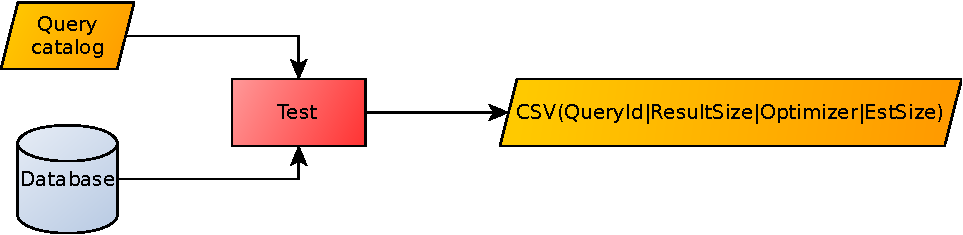
\includegraphics[width=0.9\textwidth]{figures/testbed.pdf}
  \caption{The test setting.}
  \label{fig:testbed}
\end{figure}

The platform of execution is not relevant, because the measured variables
(result size and estimated sizes) are platform-independent.

\subsection{Query Dimensions}
\label{sec:query-dimensions}

As discussed in Section \ref{sec:cypher-to-operators}, our cardinality
estimations cover all CSP queries that map to a tree subgraph pattern.
% For this query space, our test compares our estimations with the
% estimations of Neo4j.
Within this query space, we can group queries according to several
important dimensions:
\begin{samepage}
\begin{enumerate}
  \renewcommand{\labelenumii}{\theenumii}
  \renewcommand{\theenumii}{\theenumi.\arabic{enumii}.}
  \renewcommand{\theenumiii}{\theenumii\arabic{enumiii}}
  
  \item Query shapes
    \begin{enumerate}
      \item Chain queries (denoted by --)
      \item Star queries (denoted by *)
      \item Snowflake queries (denoted by \#)
    \end{enumerate}
  \item Type constraints
    \begin{enumerate}
      \item Queries without type constraints
      \item Queries with type constraints
    \end{enumerate}
  \item Label constraints
    \begin{enumerate}
      \item Queries without label constraints
      \item Queries with label constraints
      \begin{enumerate}
        \item Queries with redundant label constraints (explanation below)
        \item Queries where labels are in a sublabel relation
        \item Queries where labels are disjoint
        \item Queries where labels are (approximately) independent
      \end{enumerate}
    \end{enumerate}
\end{enumerate}
\end{samepage}

We call a label constraint on a node variable \emph{redundant}, if the label is
already determined by the type of a relationship connected to the node
variable.
E.g. in the SNB schema shown below, if a node variable is connected to an
outgoing relationship of type "HAS\_INTEREST", adding "Person" as a label
constraint on this node variable is redundant.

In order to be representative, a catalog of test queries should cover most of
the value combinations of the given dimensions.

\subsection{Dataset: The LDBC Social Network Benchmark}

According to the homepage:
\begin{quote}
"The Social Network Benchmark (SNB) consists of a data generator that generates
a synthetic social network, used in three workloads: Interactive, Business
Intelligence and Graph Analytics. Currently, only the Interactive Workload has
been released in draft stage."

(\url{http://ldbcouncil.org/developer/snb}, 06/04/2017)
\end{quote}

We use the dataset of the Interactive workload
\cite{erling_ldbc_2015} with default settings.

\subsubsection{Importing the Dataset}

After executing the data generator%
\footnote{\url{https://github.com/ldbc/ldbc_snb_datagen}, 1.6.2017}, the
generated CSV files have to be imported into Neo4j using the Neo4j import
tool%
\footnote{\url{https://neo4j.com/docs/operations-manual/3.1/tools/import/},
5.6.2017}.
The import requires a reformatting of the CSV files, which can be achieved by
Jonathan Ellithorpe's \emph{DataFormatConverter}%
\footnote{\url{https://github.com/PlatformLab/ldbc-snb-impls/blob/%
6d52ca5cc492ca8aeffed4cbbdcf7d1a6c073061/snb-interactive-neo4j/%
src/main/java/net/ellitron/ldbcsnbimpls/interactive/neo4j/util/%
DataFormatConverter.java}, 5.6.2017}.
% However, the mapping used in the DataFormatConverter uses a property "type" to
% differentiate between the subclasses of the Place and Organisation classes.
% Because we do not consider properties in our graph model, we add the
% respective labels (City, Country, Continent, University, Company) to the
% subclasses after the import.

\subsubsection{Label Partition and Sublabel Map}

The schema of the SNB data is shown in Figure \ref{fig:snb-schema}.
The mapping to a property graph performed by the \texttt{DataFormatConverter}
uses a property "type" to differentiate between the subclasses of the Place and
Organisation classes.
Because we do not consider properties in our graph model, we add the
respective labels (City, Country, Continent, University, Company) to the
subclasses after the import.
After this step, all classes in the schema map directly to node labels in
our database.

\begin{figure}
  \centering
  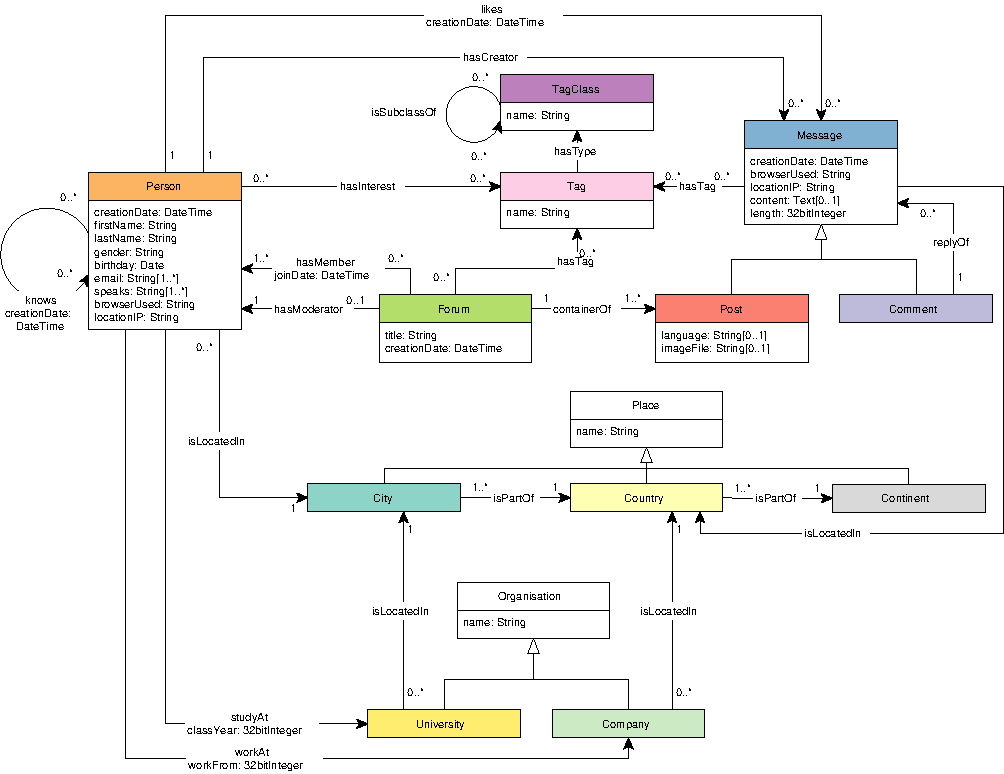
\includegraphics[width=\textwidth]{figures/snb_schema.pdf}
  \caption{Schema of the SNB Interactive workload. Taken from
  \textit{LDBC SNB Documentation 0.3.0},
  \url{https://github.com/ldbc/ldbc_snb_docs},
  06/04/2017.}
  \label{fig:snb-schema}
\end{figure}

Observe that every node in the database has at least one label.
Furthermore, any two different labels in the SNB schema are either disjoint or
in a sublabel relation.
This label distribution can be stored in a label partition and a sublabel
map, which are needed by our estimations.
We use the strict label partition and the strict sublabel map
(cf. Section \ref{sub:sublabel-map}).
The strict label partition is given as
\begin{align}
\begin{split}
  \lpart_\snb := \{ &\{ \text{Message}, \text{Post}, \text{Comment} \}, \\
                    &\{ \text{Place}, \text{Continent}, \text{Country},
                        \text{City} \}, \\
                    &\{ \text{Organisation}, \text{University},
                        \text{Company} \}, \\
                    &\{ \text{Person} \}, \\
                    &\{ \text{Forum} \}, \\
                    &\{ \text{Tag} \}, \\
                    &\{ \text{TagClass} \} \}
\end{split}
\end{align}

The strict sublabel map is given as
\begin{align}
\begin{split}
  &\submap_\snb(\text{Message}) := \{ \text{Post}, \text{Comment} \}, \\
  &\submap_\snb(\text{Post}) := \emptyset \\
  &\submap_\snb(\text{Comment}) := \emptyset \\
  &\submap_\snb(\text{Place}) := \{ \text{Continent}, \text{Country},
                                    \text{City} \}, \\
  &\submap_\snb(\text{Continent}) := \emptyset \\
  &\submap_\snb(\text{Country}) := \emptyset \\
  &\submap_\snb(\text{City}) := \emptyset \\
  &\submap_\snb(\text{Organisation}) := \{ \text{University},
                                           \text{Company} \}, \\
  &\submap_\snb(\text{University}) := \emptyset \\
  &\submap_\snb(\text{Company}) := \emptyset \\
  &\submap_\snb(\text{Person}) := \emptyset \\
  &\submap_\snb(\text{Forum}) := \emptyset \\
  &\submap_\snb(\text{Tag}) := \emptyset \\
  &\submap_\snb(\text{TagClass}) := \emptyset
\end{split}
\end{align}

\subsection{Query Catalog}

The queries contained in the  SNB Interactive workload exceed by far what we
can express in our current query algebra.
Therefore, we select a subset of interesting queries in the SNB schema and
compare the cardinality estimations of our model and Neo4j's model on this
subset.

Tables \ref{table:query-catalog-1}, \ref{table:query-catalog-2} and
\ref{table:query-catalog-3}  show our query catalog for the SNB.
For each query, the table lists the unique query id, the Cypher pattern,
the query shape and whether the query has type or label constraints.

Our query catalog covers most of the value combinations of the query dimensions
specified in Section \ref{sec:query-dimensions}.
However, due to the SNB schema, it does not occur that two labels are
(approximately) independent.

\begin{landscape}
  \begin{table}[h]
    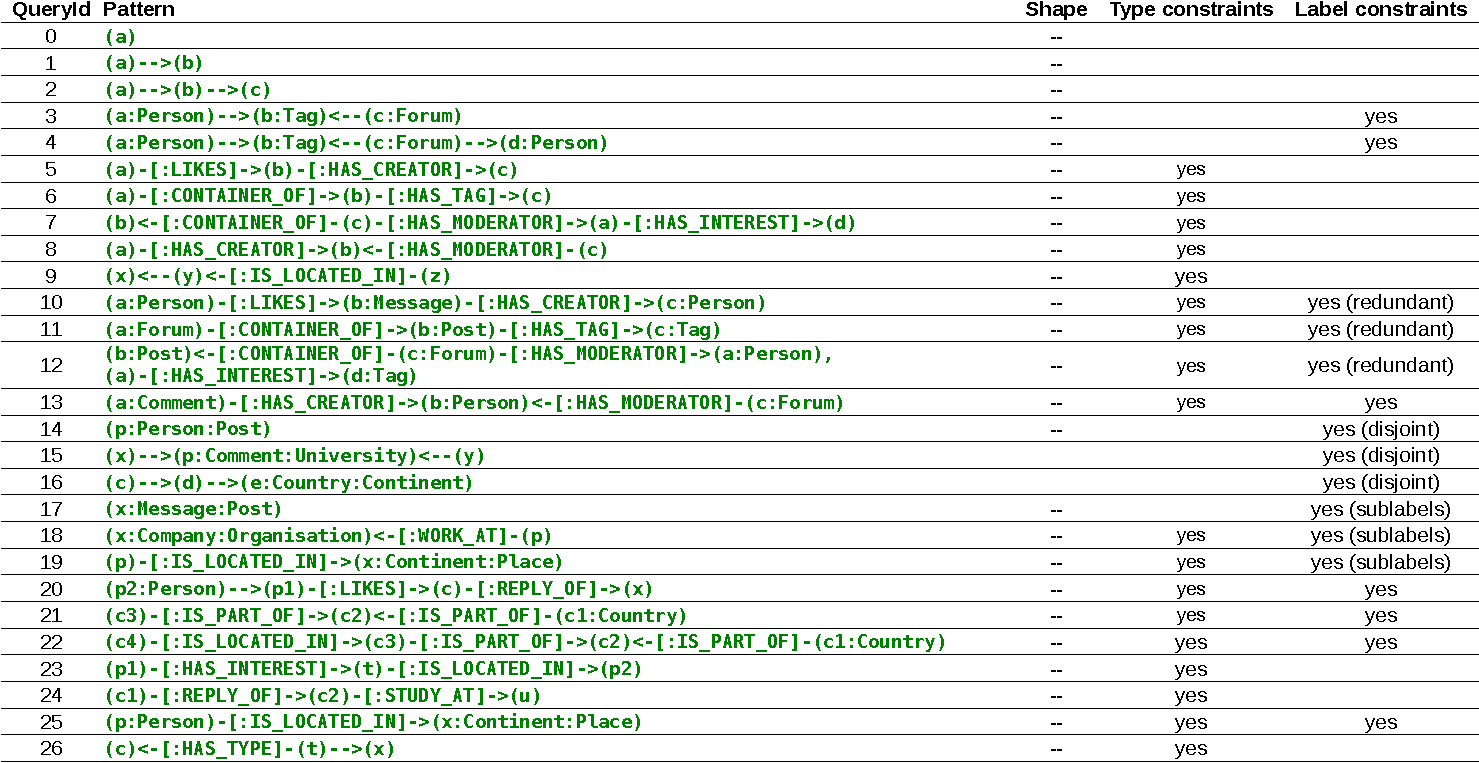
\includegraphics[width=\linewidth]{tables/snb-query-catalog/query_catalog_1.pdf}
    \caption{The catalog of test queries for the SNB (part 1).}
    \label{table:query-catalog-1}
  \end{table}
  \begin{table}[h]
    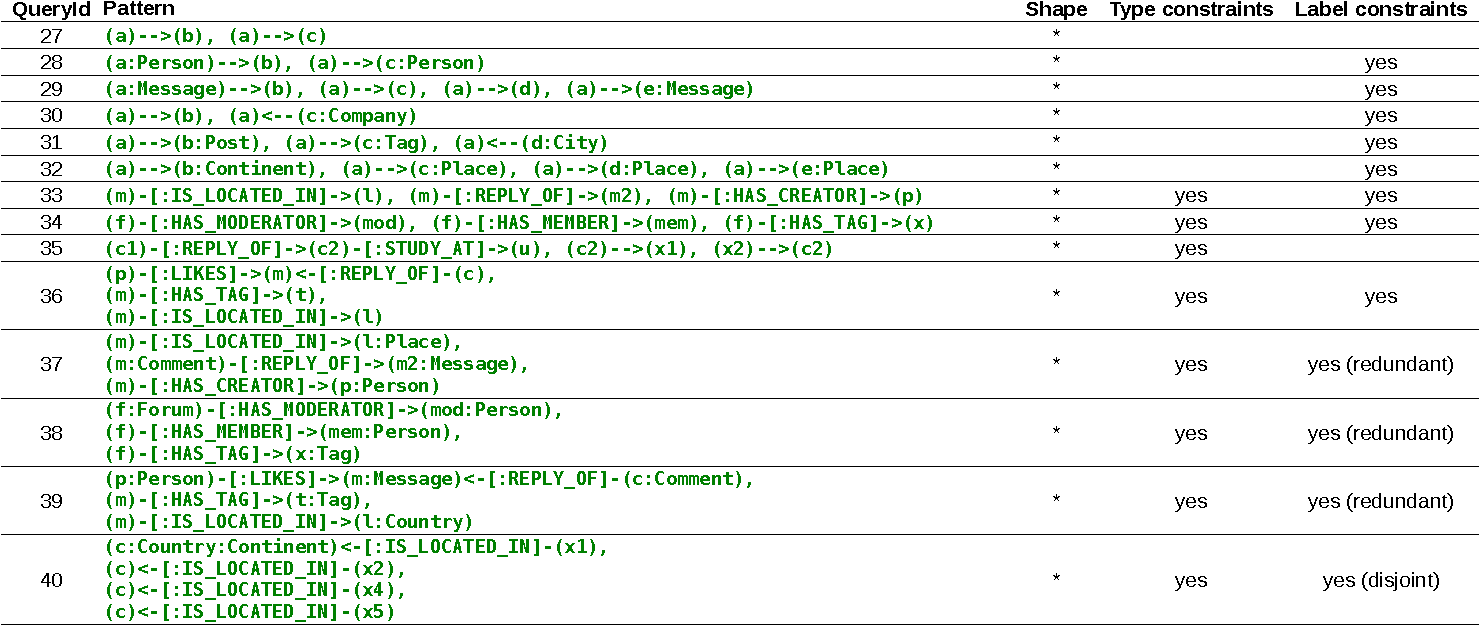
\includegraphics[width=\linewidth]{tables/snb-query-catalog/query_catalog_2.pdf}
    \caption{The catalog of test queries for the SNB (part 2).}
    \label{table:query-catalog-2}
  \end{table}
  \begin{table}[h]
    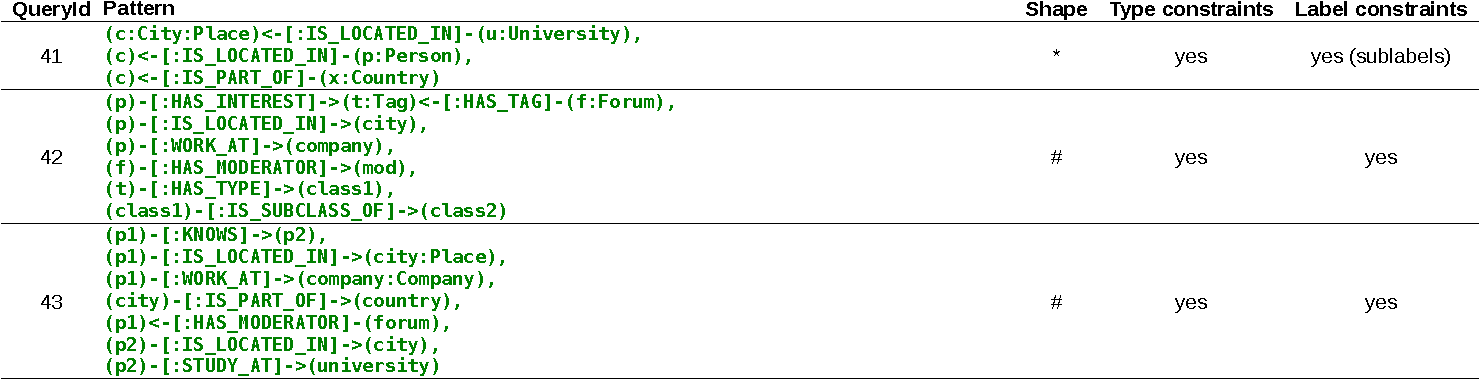
\includegraphics[width=\linewidth]{tables/snb-query-catalog/query_catalog_3.pdf}
    \caption{The catalog of test queries for the SNB (part 3).}
    \label{table:query-catalog-3}
  \end{table}
\end{landscape}

\section{Analysis}

The complete results of our tests can be found in Appendix
\ref{app:test-results}.

\subsection{Comparison of the Correlation between Actual and Estimated
            Result Cardinalities}

For any predictive model it is desirable that its predictions are strongly
linearly correlated with the actual observations.
A strong linear correlation means that, the model behaves like reality
(apart from a constant shift and rescaling).

For our cardinality estimations, a strong linear correlation
between the actual result cardinality and the estimated cardinality
implies for instance that, if query A has a smaller result cardinality than
query B, the estimated cardinality of A will probably also be smaller than
the estimated cardinality of B.
This property is crucial for any optimizer, in order to choose the execution
plan where the intermediate cardinalities are minimal.

Our hypothesis is that, our estimations are \emph{significantly}
more correlated with the actual result cardinalities than Neo4j's estimations,

In order to prove this hypothesis, we have to use statistical tests.
We compute these tests in R, using the \emph{cocor} package%
\cite{diedenhofen_cocor:_2015}%
\footnote{\url{https://cran.r-project.org/web/packages/cocor/index.html},
18.06.2017}.
Cocor computes several tests at once, including Pearson and Filon's z-test.

In the following R code, the variables have the following meaning:
\begin{itemize}
  \item \texttt{ResultSize} is the actual result cardinality of a query.
  \item \texttt{Neo4jEstSize} is Neo4j's estimate of the result cardinality
    of a query.
  \item \texttt{CascadesEstSize} is our estimate of the result cardinality
    of a query.
\end{itemize}

We want to show that our estimations correlate better with the actual result
cardinalities than the estimations of Neo4j.

The corresponding null hypothesis is that, the correlation between
\texttt{ResultSize} and \texttt{Neo4jEstSize} is greater or equal than
the correlation between
\texttt{ResultSize} and \texttt{CascadesEstSize}.

The following R statement runs the test:
\begin{verbatim}
cocor(~ResultSize + EstNeo4j | ResultSize + EstCascades,
      t, alternative = "less", conf.level = 0.99)
\end{verbatim}

The test output tells us, that the actual result cardinality
is only marginally correlated with the estimations of Neo4j ($r = 0.0409$),
but strongly correlated with our estimations ($r = 0.8258$).

Moreover, Table \ref{table:cocor-test-results} shows that all tests run by
cocor tell us to reject our null hypothesis at 99\% confidence level
($\alpha = 0.01$)%

\begin{table}
\centering
\caption{Formatted output of the tests run by cocor.}
\label{table:cocor-test-results}
\begin{tabular}{@{}lll@{}}
\toprule
Test name                                                                                                                                                                             & Test result                                                                                           & \begin{tabular}[c]{@{}l@{}}Null\\ hypothesis\\ rejected?\end{tabular} \\ \midrule
Pearson and Filon's z (1898)                                                                                                                                                          & \begin{tabular}[c]{@{}l@{}}z = -4.8927\\ p-value = 0.0000\end{tabular}                                & Yes                                                                   \\
Hotelling's t (1940)                                                                                                                                                                  & \begin{tabular}[c]{@{}l@{}}t = -6.2367\\ df = 41\\ p-value = 0.0000\end{tabular}                      & Yes                                                                   \\
Williams' t (1959)                                                                                                                                                                    & \begin{tabular}[c]{@{}l@{}}t = -5.4285\\ df = 41\\ p-value = 0.0000\end{tabular}                      & Yes                                                                   \\
Olkin's z (1967)                                                                                                                                                                      & \begin{tabular}[c]{@{}l@{}}z = -4.8927\\ p-value = 0.0000\end{tabular}                                & Yes                                                                   \\
Dunn and Clark's z (1969)                                                                                                                                                             & \begin{tabular}[c]{@{}l@{}}z = -4.9999\\ p-value = 0.0000\end{tabular}                                & Yes                                                                   \\
\begin{tabular}[c]{@{}l@{}}Hendrickson, Stanley, and Hills' (1970)\\ modification of Williams' t (1959)\end{tabular}                                                                  & \begin{tabular}[c]{@{}l@{}}t = -6.2169\\ df = 41\\ p-value = 0.0000\end{tabular}                      & Yes                                                                   \\
\begin{tabular}[c]{@{}l@{}}Steiger's (1980) modification of Dunn\\ and Clark's z (1969) using average correlations\end{tabular}                                                       & \begin{tabular}[c]{@{}l@{}}z = -4.8416\\ p-value = 0.0000\end{tabular}                                & Yes                                                                   \\
Meng, Rosenthal, and Rubin's z (1992)                                                                                                                                                 & \begin{tabular}[c]{@{}l@{}}z = -4.7835\\ p-value = 0.0000\end{tabular}                                & Yes                                                                   \\
\begin{tabular}[c]{@{}l@{}}Hittner, May, and Silver's (2003) modification of\\ Dunn and Clark's z (1969) using a\\ backtransformed average Fisher's (1921)\\ Z procedure\end{tabular} & \begin{tabular}[c]{@{}l@{}}z = -4.7825\\ p-value = 0.0000\end{tabular}                                & Yes                                                                   \\
Zou's (2007) confidence interval                                                                                                                                                      & \begin{tabular}[c]{@{}l@{}}99\% confidence\\ interval for r.jk - r.jh:\\ -1.1878 -0.3610\end{tabular} & Yes                                                                   \\ \bottomrule
\end{tabular}
\end{table}


We can therefore conclude that our estimations are
significantly stronger correlated with the actual result size than Neo4j's
estimations.

The complete test output can be found in Appendix \ref{app:cocor-r-snippet}.

\subsection{Comparison of the Estimation Errors}
\label{sec:estimations-errors}

The predictions produced by a model should not only have a strong linear
correlation with real observations, they should also be \emph{close} to the
observations with respect to some error metric.
For our model, we use the \emph{absolute estimation error} and the
\emph{relative estimation error} as error metrics.

\begin{definition}[Absolute and relative estimation error]
Take a CSP query $c$ with result cardinality $x$.
Suppose an optimizer estimates the result cardinality of $c$ as $\hat{x}$.
The absolute error of this estimation is defined as
\[
  \absErr(x, \hat{x}) := | x - \hat{x} |
\]

If $x \not = 0$, the relative error of this estimation is defined as
\[
  \relErr(x, \hat{x}) := \frac{\absErr(x, \hat{x})}{| x |}
\]
\end{definition}

To decide whether there is a significant difference between the estimation
errors of the optimizers, we use the test for paired observations described by
Raj Jain \cite[p.~209]{jain_art_1991}.

For each query of the catalog, we observe the (absolute/relative) estimation
error of both optimizers. For each pair of error observations, we compute the
difference. Then we compute a confidence interval for this difference.
If this confidence interval includes zero, the systems are not significantly
different. If it does not include zero, there is a significant difference
between the (absolute/relative) estimation errors of the optimizers.

% \subsubsection{Comparison With Respect to Query Dimensions}
%
% Using our specified query dimensions, we try to find subsets where the
% (absolute/relative) estimation error of our and Neo4j's estimation model
% differ the most.
%
\subsubsection{Absolute Estimation Error}

Figure \ref{fig:abs-error-snb} shows the absolute estimation error $\epsilon$
of the two estimation models for the queries in the SNB query catalog.
We transform the error scale using the inverse hyperbolic sine%
\footnote{The inverse hyperbolic sine transformation (asinh) allows to cover
many orders of magnitude and is defined for all real numbers.
cf. \url{http://wresch.github.io/2013/03/08/asinh-scales-in-ggplot2.html},
18.06.2017},
because the error values vary by several orders of magnitude.
The figure indicates that our estimations generate the smaller absolute errors.

\begin{figure}
  \centering
  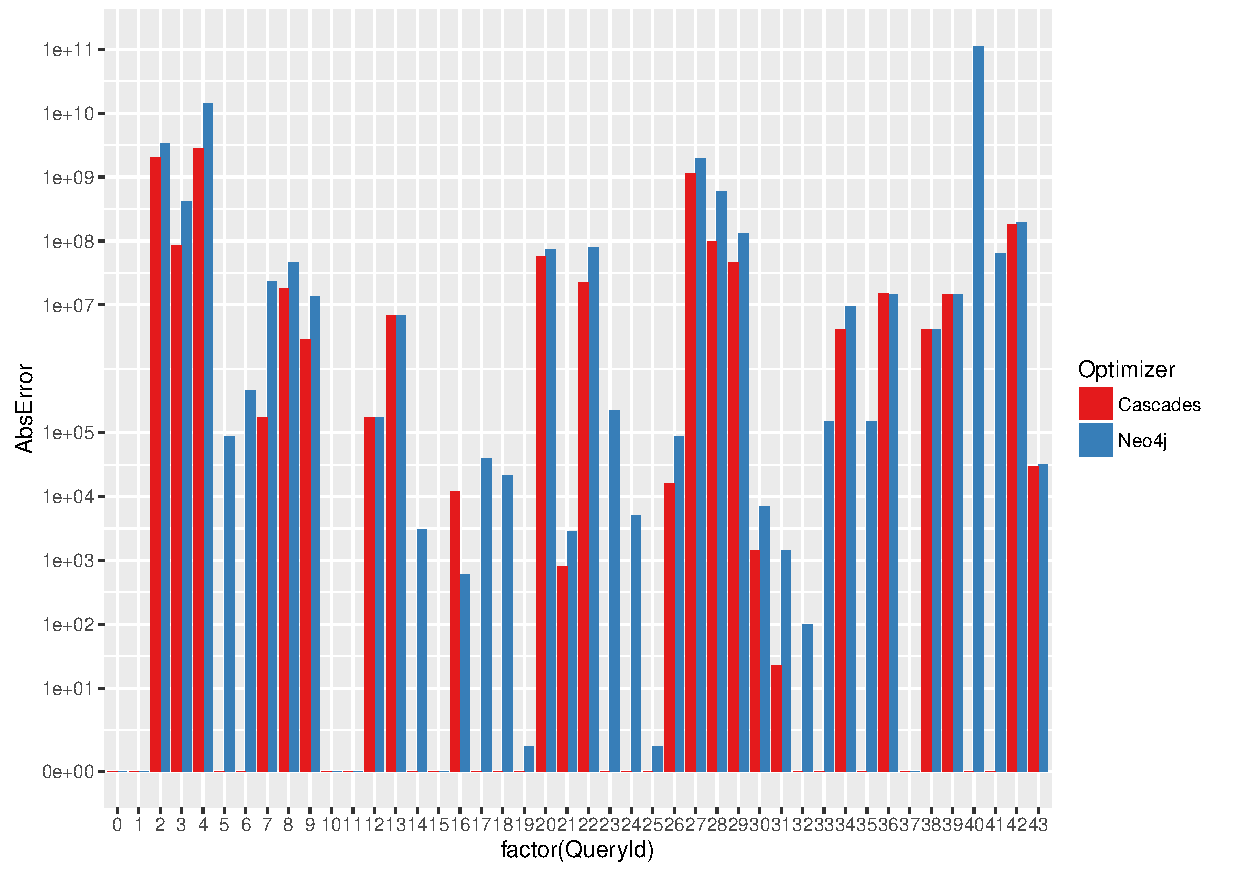
\includegraphics[width=\textwidth]{figures/eval/abs_error_snb.pdf}
  \caption{Absolute errors of our estimations (Cascades, \emph{red})
           and Neo4j's estimations (Neo4j, \emph{blue})
           for the SNB query catalog.}
  \label{fig:abs-error-snb}
\end{figure}

Figure \ref{fig:abs-error-diff-snb} shows the difference $d_\epsilon$
between the absolute
error of Neo4j's estimations and the absolute error of our estimations.
Like above, we transform the scale using the inverse hyperbolic sine.
Again, we see that our estimations generate the smaller absolute
errors for most of the queries in question.

\begin{figure}
  \centering
  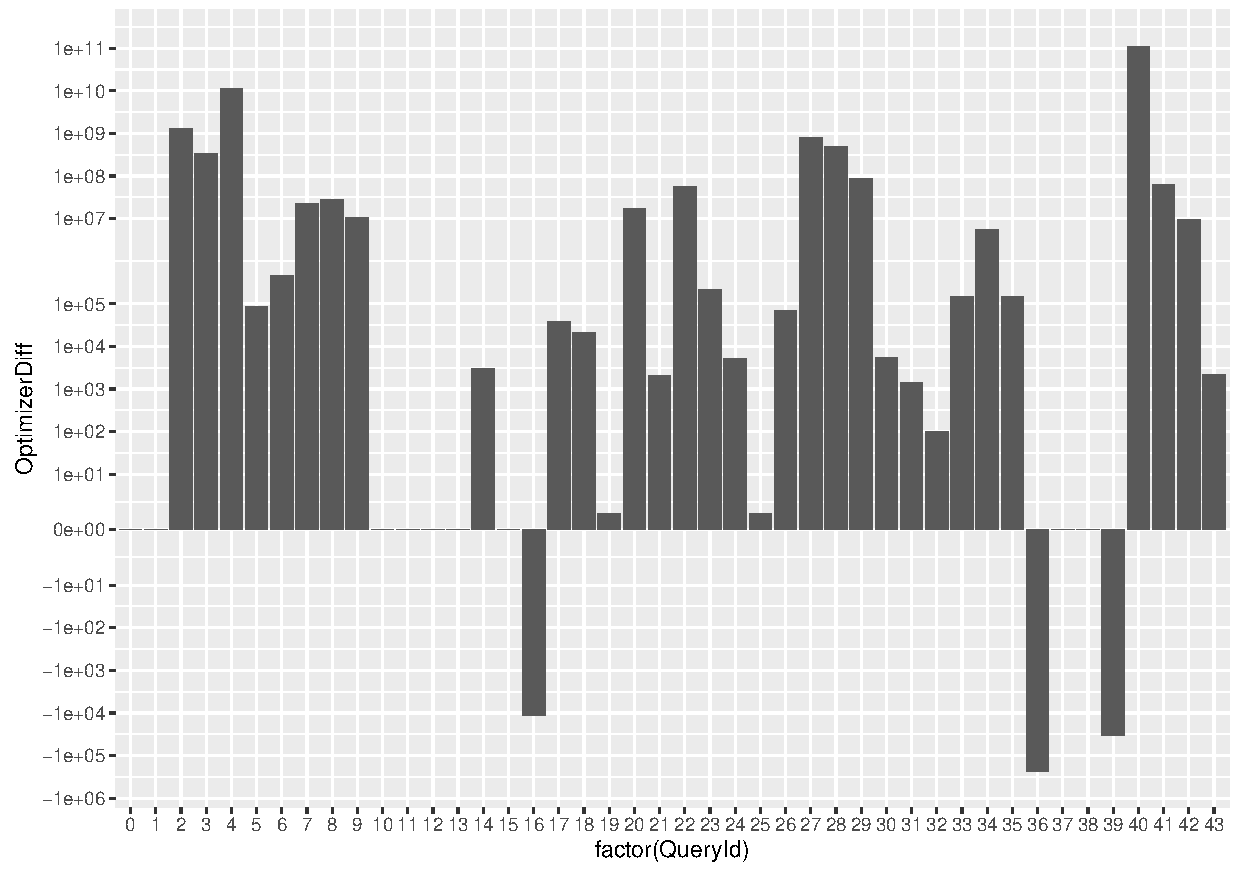
\includegraphics[width=\textwidth]{figures/eval/abs_error_diff_snb.pdf}
  \caption{Difference between the absolute error of Neo4j's estimations
           and our estimations for the SNB query catalog.}
  \label{fig:abs-error-diff-snb}
\end{figure}

Table \ref{table:abs-error-diff-stats} shows that
on average, our estimations are $2\,869\,783\,102$ subgraphs closer to the
actual result cardinality than the estimations of Neo4j.

\begin{table}[h]
\centering
\begin{tabular}{@{}lll@{}}
\toprule
n  & $\text{mean}(d_\epsilon)$    & $\text{var}(d_\epsilon)$ \\ \midrule
44 & $2\,869\,783\,102$           & $2.850809 \cdot 10^{20}$ \\ \bottomrule
\end{tabular}
\caption{Sample size, mean and variance of $d_\epsilon$.}
\label{table:abs-error-diff-stats}
\end{table}

In order to test whether the observed difference in absolute errors is already
\emph{significant}, we compute the 99\% confidence interval of $d_\epsilon$
using the simple procedure described by Raj Jain \cite[p.~209]{jain_art_1991}.
Let $t(0.99, n-1)$ denote the $0.99$-quantile of a t-variate with $n-1$
degrees of freedom. Then the confidence interval $c_\epsilon$ is
\begin{align}
\begin{split}
  c_\epsilon &= \text{mean}(d_\epsilon) \pm t(0.99, n - 1)
                 \cdot \sqrt{\frac{\text{var}(d_\epsilon)}{n}} \\
             &= 2869783102 \pm 2.41625
                \cdot \sqrt{\frac{2.850809 \cdot 10^{20}}{44}} \\
             &\approx (-3280563476.14, 9020129680.14)
\end{split}
\end{align}

This confidence interval includes zero. Consequently, our current SNB query catalog
is not sufficient to conclude that our estimations have significantly smaller absolute
estimation errors than Neo4j's estimations.

To be able to prove this in future experiments, we should increase the sample
size (i.e., the number of queries in the catalog) in order to decrease the
variance of $d_\epsilon$ and thus reduce the size of the confidence interval.

\subsubsection{Relative Estimation Error}

The relative estimation error $\eta$ is only defined for queries having a
non-empty result. In our query catalog, these are 31 queries.
Figure \ref{fig:rel-error-snb} shows the relative estimation error
of our and Neo4j's estimation model for these queries.
The figure indicates that our estimations generate the smaller relative errors.

\begin{figure}
  \centering
  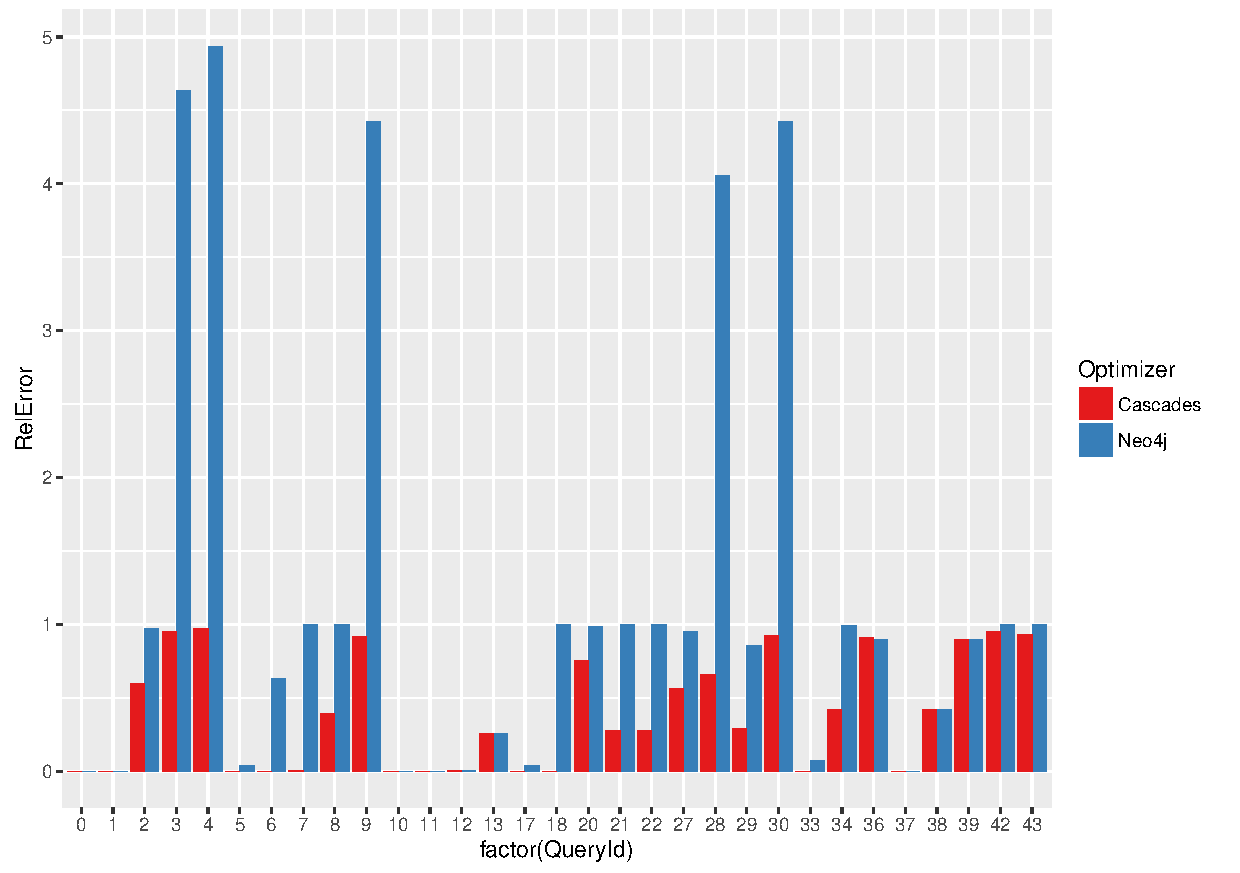
\includegraphics[width=\textwidth]{figures/eval/rel_error_snb.pdf}
  \caption{Relative errors of our estimations (Cascades, \emph{red})
           and Neo4j's estimations (Neo4j, \emph{blue})
           for the SNB query catalog.}
  \label{fig:rel-error-snb}
\end{figure}

Figure \ref{fig:rel-error-diff-snb} shows the difference $d_\eta$
between the relative
error of Neo4j's estimations and the relative error of our estimations.
Again, we see that our estimations generate the lower relative
errors for most of the queries.

\begin{figure}
  \centering
  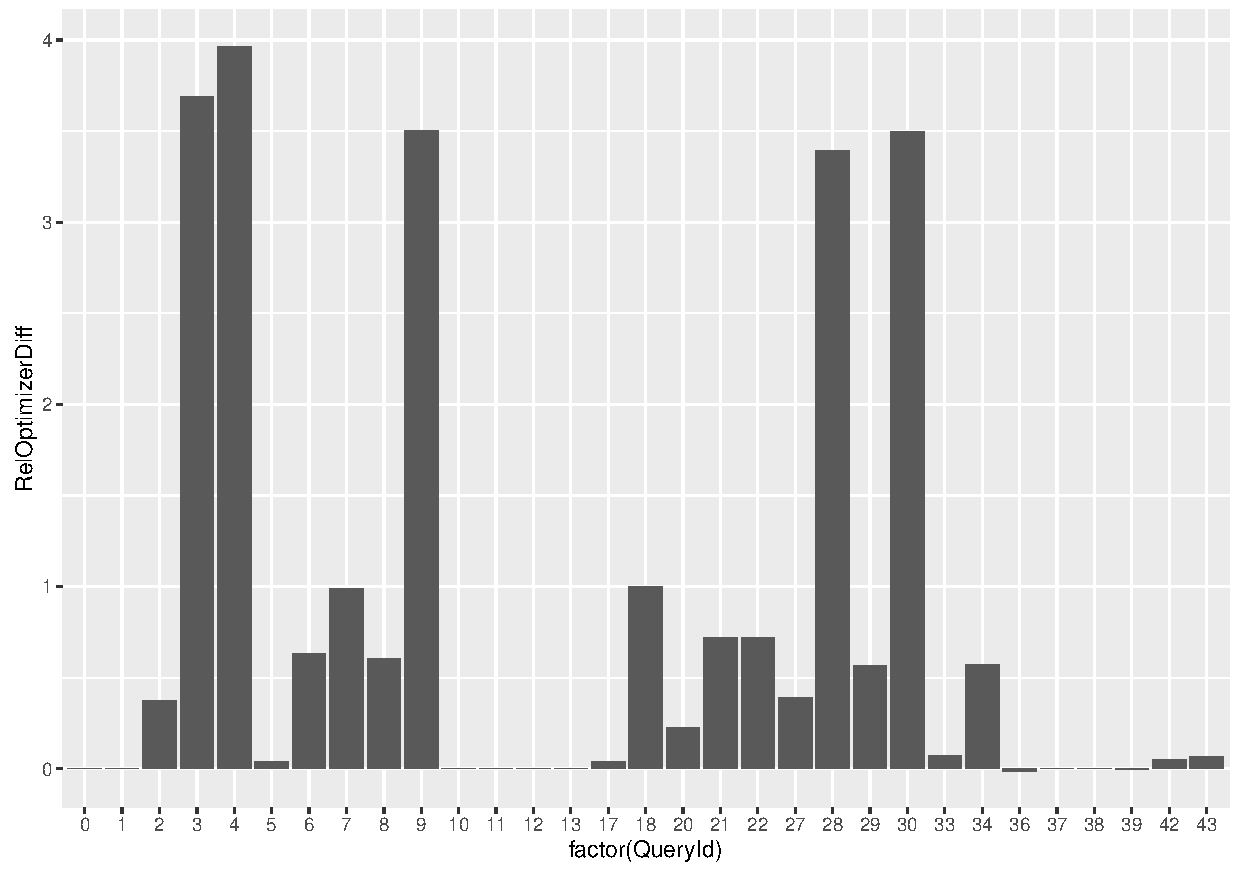
\includegraphics[width=\textwidth]{figures/eval/rel_error_diff_snb.pdf}
  \caption{Difference between the relative error of Neo4j's estimations
           and our estimations for the SNB query catalog.}
  \label{fig:rel-error-diff-snb}
\end{figure}

Table \ref{table:rel-error-diff-stats} shows that
on average, our relative estimation error is $0.8096792$ smaller than
the relative estimation error of Neo4j.

\begin{table}[h]
\centering
\begin{tabular}{@{}lll@{}}
\toprule
n  & $\text{mean}(d_\eta)$ & $\text{var}(d_\eta)$ \\ \midrule
31 & $0.809679$          & $1.661361$             \\ \bottomrule
\end{tabular}
\caption{Sample size, mean and variance of $d_\eta$.}
\label{table:rel-error-diff-stats}
\end{table}

In order to test whether the observed difference in relative errors is already
\emph{significant}, we compute the 99\% confidence interval of $d_\eta$ using
the same procedure as above.
The confidence interval $c_\eta$ is
\begin{align}
\begin{split}
  c_\eta &= \text{mean}(d_\eta) \pm t(0.99, n - 1)
            \cdot \sqrt{\frac{\text{var}(d_\eta)}{n}} \\
         &= 0.809679 \pm 2.452824
            \cdot \sqrt{\frac{1.661361}{31}} \\
         &\approx (0.24185, 1.377507)
\end{split}
\end{align}

This confidence interval is located above zero.
Hence, we can conclude by 99\% significance that our estimations generate
smaller relative errors than Neo4j's estimations.



\chapter{Summary}

In this thesis, we have layed some important groundwork for sophisticated graph
query optimization.

% What have we done
%  theoretical work
%  evaluation
% 
% What are the current limitations
% What is future work

\paragraph{A Graph Query Algebra}

We have formally introduced a query
algebra for graph databases, extending the algebra of Hölsch et al.%
\cite{holsch_algebra_2016} (cf. Chapter \ref{chap:query-algebra}).
We have proven that this graph algebra is well-defined and complete.
Currently, our graph algebra allows to express subgraph matching with label,
type and uniqueness constraints, which is an essential part of any
graph query language.

\paragraph{A Statistical Model to Estimate Result Cardinality}

Moreover, we have illustrated that a global assumption on the distribution of node
labels in a graph database can lead to severe estimation errors for datasets
where this assumption is violated.
We have introduced two new data structures, the \emph{label partition} and the
\emph{sublabel map}, to address this problem.

We have then implemented our own cardinality estimation model in the Neo4j
graph database.
The model provides cardinality estimations for a subset of operators of our
graph algebra, namely for the \op{GetNodes}, \op{Expand} and
\op{NodeLabelSelection} operators
(cf. Section \ref{sec:cypher-to-operators} for the corresponding subset of
Cypher).
For each of these operators, we have explained in detail, which assumptions
lead to the respective estimation function.
Our model uses similar database statistics as Neo4j, plus a label partition and a
sublabel map. Using the information provided by these two data structures, our
model can avoid estimation errors if labels are not independent.
Furthermore, by keeping track of the \emph{label probabilities} at each node
variable of the query pattern, our model is able to deal with strong
dependencies between node labels and the presence of relationships.

We have compared our estimation model to the estimation model of Neo4j
in a statistical analysis. On a catalog of 44 queries about the LDBC Social
Network Benchmark (SNB)\cite{erling_ldbc_2015}, our estimations are
significantly more correlated with the actual result sizes than the
estimations of Neo4j. Our model also has significantly lower relative
estimation errors.

\chapter{Future Work}

\paragraph{Generalizing the Graph Algebra}

We believe that a general graph query algebra is a powerful
mathematical tool to design new graph query optimizers and to analyze the variety
of existing graph databases using a common language.
This motivation has led to the first version of the graph algebra in this thesis.
In the future, we want to extend our algebra to cover more use cases,
e.g. result projections and shortest-paths queries.

\paragraph{Conducting More Tests}

The tests of our model for graph query cardinality estimation have revealed,
that it correlates better with the actual result sizes and generates lower relative
estimation errors than Neo4j's current model on a catalog
of 44 queries about the SNB.
To prove that our model also has the lower absolute estimation errors, we will have
to increase the size of the query catalog.
We will also conduct similar tests on other datasets (e.g. the Movie Database%
\footnote{\url{https://neo4j.com/developer/movie-database/}}) to prove the general
superiority of our estimation model.

\paragraph{Extending the Query Space of the Estimation Model}

Currently, our estimation model is only defined for
a very limited query space (cf. Section \ref{sec:query-restrictions}).
In the future, we want to extend the query space covered by the model by
defining estimation functions for the remaining operators \op{Traverse},
\op{DistinctSelection} and \op{NodeJoin}. The estimation function for the
\op{Traverse} operator requires statistics about the likeliness of cycles in
the database graph. Defining and implementing these statistics is thus a
necessary next step to complete our estimation model.

\paragraph{An Algorithm to Update the Label Partition and the Sublabel Map
           Online}

Our estimation model is informed by a label partition and a sublabel map to
avoid estimation errors if labels are not independent. While we have illustrated
methods to generate these data structures \emph{offline}, it remains an open
research question how they can be updated \emph{online} in the presence of
database updates.
The design of an online algorithm to update the label partition and the
sublabel map is needed to make our estimation model suitable for
update-intensive graph database applications.

\paragraph{Designing the Remaining Parts of the Cascades Query Optimizer}

As mentioned in the Introduction, the estimation model proposed in this thesis
is planned as a part of a new query optimizer for graph databases that will be
implemented in the Cascades framework\cite{graefe_cascades_1995}.
In the future, we want to design and implement the remaining parts of this
optimizer. Firstly, we have to define \emph{physical operators} that are
able to produce the results of combinations of our logical operators in a
specific graph DBMS.
Secondly, we  have to design a \emph{cost model} to estimate the
memory and CPU costs of these operators.
Thirdly, we have to define a complete set of equivalence rules on the
graph query algebra, which can then be used by the Cascades optimizer to
explore the query space.

\paragraph{Combining Research on Graph and Relational Databases}

As a final remark we want to emphasize that,
cardinality estimation in graph databases
and relational databases poses very similar problems. We belief that, much of
the research that has led to todays relational optimizers is also relevant to
graph databases and should not be overlooked. As detailed above, we consider a
general graph query algebra
(motivated by the relational algebra) and a modular, algebraic graph query
optimizer (motivated by the Cascades optimizer for relational databases)
to be promising research areas for the advancement of graph databases.

Inversely, we are also convinced that insights from graph database research can
help to solve current problems of relational databases.
For instance, Guy Lohman states that estimating the
\emph{selectivity of join predicates} is a major issue in  current relational
databases\footnote{\url{http://wp.sigmod.org/?p=1075}, 24.06.2017}.
A relational join can be translated to a relationship matching in a graph database and the
join predicate can often be translated to a constraint on the relationship
type.
Translating the triple statistics maintained in graph databases (number of
relationships of a particular type between nodes having particular labels) to
triple statistics for relational databases (cardinality of a join between two
tables using a particular predicate) could allow to use our graph query
estimation model in a relational database and potentially improve the
state-of-the-art of relational cardinality estimation.

We believe that there are many "low-hanging fruits" for researchers that simply
require some transfer between the relational and graph database communities.


\appendix
\chapter{Appendix}

\section{Estimation Results}
\label{app:test-results}

The following Table \ref{table:test-results} lists the actual and estimated result
cardinality of our ("Cascades") and Neo4j's ("Neo4j") estimation model for all
queries of our SNB query
catalog (cf. Tables  \ref{table:query-catalog-1}, \ref{table:query-catalog-2} and
\ref{table:query-catalog-3}).

\begin{longtable}{llll}
\label{table:test-results} \\
\toprule
\midrule
Query Id & Result cardinality & Optimizer & Estimated cardinality \\
\midrule
\endfirsthead
\midrule
Query Id & Result cardinality & Optimizer & Estimated cardinality \\
\midrule
\endhead
\caption{Result cardinalities and
         estimated cardinalities
         for the SNB query catalog.}
\endfoot
\bottomrule
\endlastfoot
\csvreader[separator=pipe,
           head to column names,
           late after line=\\]{queries/snb/sizesAndEstimations.csv}{}%
{ \QueryId & \ResultSize & \Optimizer & \EstSize }
\end{longtable}

\section{R Output of the Correlation Test}
\label{app:cocor-r-snippet}

\begin{verbatim}
  Results of a comparison of two overlapping
  correlations based on dependent groups

Comparison between r.jk (ResultSize, EstNeo4j) = 0.0409
               and r.jh (ResultSize, EstCascades) = 0.8258
Difference: r.jk - r.jh = -0.7848
Related correlation: r.kh = -0.0374
Data: t: j = ResultSize, k = EstNeo4j, h = EstCascades
Group size: n = 44
Null hypothesis: r.jk is equal to r.jh
Alternative hypothesis: r.jk is less than r.jh (one-sided)
Alpha: 0.05

pearson1898: Pearson and Filon's z (1898)
  z = -4.8927, p-value = 0.0000
  Null hypothesis rejected

hotelling1940: Hotelling's t (1940)
  t = -6.2367, df = 41, p-value = 0.0000
  Null hypothesis rejected

williams1959: Williams' t (1959)
  t = -5.4285, df = 41, p-value = 0.0000
  Null hypothesis rejected

olkin1967: Olkin's z (1967)
  z = -4.8927, p-value = 0.0000
  Null hypothesis rejected

dunn1969: Dunn and Clark's z (1969)
  z = -4.9999, p-value = 0.0000
  Null hypothesis rejected

hendrickson1970: Hendrickson, Stanley, and Hills' (1970)
                 modification of Williams' t (1959)
  t = -6.2169, df = 41, p-value = 0.0000
  Null hypothesis rejected

steiger1980: Steiger's (1980) modification of Dunn and Clark's z
             (1969) using average correlations
  z = -4.8416, p-value = 0.0000
  Null hypothesis rejected

meng1992: Meng, Rosenthal, and Rubin's z (1992)
  z = -4.7835, p-value = 0.0000
  Null hypothesis rejected
  99% confidence interval for r.jk - r.jh: -1.7443 -0.5232
  Null hypothesis rejected (Upper boundary < 0)

hittner2003: Hittner, May, and Silver's (2003) modification of Dunn
             and Clark's z (1969) using a backtransformed average
             Fisher's (1921) Z procedure
  z = -4.7825, p-value = 0.0000
  Null hypothesis rejected

zou2007: Zou's (2007) confidence interval
  99% confidence interval for r.jk - r.jh: -1.1878 -0.3610
  Null hypothesis rejected (Upper boundary < 0)
\end{verbatim}

The line \texttt{Alpha: 0.05} is probably a bug in cocor. It should be
\texttt{Alpha: 0.01} to match the confidence level which was specified by the
parameter \texttt{conf.level=0.99}.


% Bibliography
% ------------

\bibliography{literature/literature}
\bibliographystyle{abbrv}

\end{document}
